
\documentclass[draft2.tex]{subfiles} 
\begin{document} 

\section{Methods} 
\label{sec:methods} 
To fulfill the goals of this paper, we develop and make use of newly released 
features within the~\texttt{Versatile Integrator for Chemical Evolution} 
(\vice;~\citealp{Johnson2020}), an open-source~\texttt{python} package 
available for~\texttt{Unix} system architectures (for further details, see 
Appendix~\ref{sec:vice}). 
These features are designed to handle models such as these with a wide range of 
flexibility. 
We reserve a description of~\vice's migration algorithm and our simulation 
parameters for~\S~\ref{sec:methods:migration}, first describing our sample of 
star particles from the hydrodynamic simulation. 
\par 
Although we make use of a hydrodynamic simulation to drive stellar migration, 
we do~\textit{not} make use of its SFH. 
While our study employs similar techniques as~\citet{Minchev2013}, ours differs 
slightly in that they take a single SFH which is similar, but not identical to 
that of their N-body+SPH simulation; in this paper we present a handful of 
assumptions about the SFH, which do not necessarily resemble that of~\hsim. 
An alternative to modeling radial migration based on a 
hydrodynamical simulation is to invoke dynamical arguments; 
\citet{Schoenrich2009a} and~\citet{Sharma2020} take such an approach. 
This method, however, introduces free parameters which then require fitting to 
data. 
An advantage of our technique is that there are no free parameters describing 
radial migration introduced to the model; it is unclear how much 
fitting radial migration parameters could bias the model into agreement with 
parts of the data not involved in the fitting process. 
Instead we adopt a physically motivated migration model evolved from 
cosmological initial conditions. 
We rely on a single realization of this numerical model and are thus subject to 
the differences between the dynamical history of this simulated galaxy and that 
of the Milky Way. 
However, one could compare the predictions made by our chemical evolution 
models when applied to different hydrodynamical simulations, a direction we 
plan to pursue in future work. 
We emphasize that the hydrodynamical simulation~\textit{only} informs the 
mixing processes in our models, and there is no N-body integration involved in 
our models aside from that which was used to run the~\hsim~simulation in the 
first place. 
{\color{red} 
A summary of our chemical evolution model parameters can be found in 
Table~\ref{tab:params}. 
} 

\subsection{The Hydrodynamical Simulation} 
\label{sec:methods:h277} 
In this paper we make use of star particles from the~\texttt{h277} simulation 
\citep{Christensen2012, Zolotov2012, Loebman2012, Loebman2014, Brooks2014}. 
Recently employed to study the stellar age-velocity relationship, a synopsis of 
its detailed simulation parameters and cosmological model can be found in~\S~2 
of~\citet{Bird2021}. 
We do not repeat these details here, instead focusing on how we vet the sample 
of star particles for use in our chemical evolution models. 
\par 
The parameters of stars that we use in our analysis are the birth and final 
radii and the final midplane distance. 
{\color{red}\textit{
	We emphasize that these are the only quantities from~\hsim~which we make 
	use of in our model; our Galaxies have their own star formation histories, 
	nucleosynthetic yields, outflow prescriptions, etc.
}}
\hsim~did not record the exact birth radius of each star particle; however, 
each star particle does have an accurate age at each snapshot. 
The orbital radii of stars that are sufficiently young in their first snapshot 
should be good approximations of their birth radii. 
We therefore restrict our sample to those star particles with an age at first 
snapshot of~$\leq$~150 Myr, and we adopt their Galactocentric radius at that 
time as their birth radius. 
We have repeated our analysis with a maximum age at first snapshot of 50 
Myr and found similar results, indicating that these time intervals are short 
enough to not impact our conclusions. 
We adopt the 150 Myr interval because it provides a larger number of star 
particles to sample from. 
Of the star particles that remain after imposing this cut, the oldest has an 
age of 13.23 Gyr at the present day (i.e. at the simulation's final output). 
Our GCE model can only apply on timescales as long as or shorter than the full 
range of ages of the sample of star particles; we therefore subtract 0.5 Gyr 
from the formation times of all star particles, allowing~$T$~= 0 in our models 
to correspond to~$T$~= 0.5 Gyr in~\hsim. 
As a consequence, our disc models trace the chemical evolution of the Galaxy 
out to a lookback time of~$\sim$13.2 Gyr, or a redshift of~$z \approx$~9, 
placing the onset of star formation at that time. 
\par 
We further restrict our sample of star particles to only those with both 
formation and final radii of~$\rgal \leq$~20 kpc, and to have formed 
within~$\absz\leq$~3 kpc of the disc midplane. 
These criteria are intended to restrict our sample to star particles that 
formed within the disc and can therefore be described by a disc GCE model. 
While it is possible that some star particles formed in a dwarf galaxy happen 
to satisfy our geometrical cuts at the star's formation time, these particles 
are few in number, and are only relevant at large~$\rgal$ and high 
ages: a region of parameter space where few stars form anyway. 
\par 
Based on a kinematic decomposition performed on the present-day phase space 
distribution of the~\texttt{h277} star particles conducted with the 
\texttt{analysis.decomp} routine within the~\texttt{pynbody} package 
\citep{pynbody}, we classify each star particle as having thin disc, thick 
disc, bulge, pseudobulge, or halo-like kinematics.
Details on the decomposition process can be found in~\citet{Brook2012} 
and~\citet{Bird2013}. 
We include the entire sample in~\vice's public code base, but make use of only 
those with disc-like kinematics in this paper. 
Our geometric selection yields 3,152,211 star particles in total, 1,751,765 of 
which have disc-like kinematics and are included in our sample. 
% Based on a kinematic decomposition performed on the present-day phase space 
% distribution of the~\texttt{h277} star particles, we include all those with 
% bulge, pseudobulge, and disc-like kinematics, excluding halo stars. 
% While we are not modeling the evolution of the bulge here, these star particles 
% are overwhelmingly located at~$\rgal\leq$~3 kpc at the present day 
% and therefore do not enter our analysis and observational comparisons below. 
% These cuts yield a sample of 3,102,519 star particles from~\hsim. 
\par 
\hsim~had a weak and transient bar during its evolution, but it does not have 
one at~$z$~= 0. 
This is a noteworthy difference between our model and that of 
\citet{Minchev2013}, and by extension the~\citet{Minchev2014, Minchev2017} 
studies as well, because they selected a hydrodynamic simulation of a galaxy 
specifically so that it would have a strong bar at~$z$~= 0. 
This could mean that the dynamical history of our model Galaxy differs from 
that of~\citet{Minchev2013} and perhaps the Milky Way itself. 
However, the difference is likely within the uncertainties of the current 
understanding of the Milky Way's dynamical history. 
Although an investigation of the impact of bar evolution on stellar migration 
and thus chemical evolution is outside the scope of this paper, it is an 
interesting question that can be probed by simply swapping the~\hsim~data 
within~\vice~for another simulation, then rerunning our numerical models and 
comparing the results. 

% fig 1 
\begin{figure*} 
\centering 
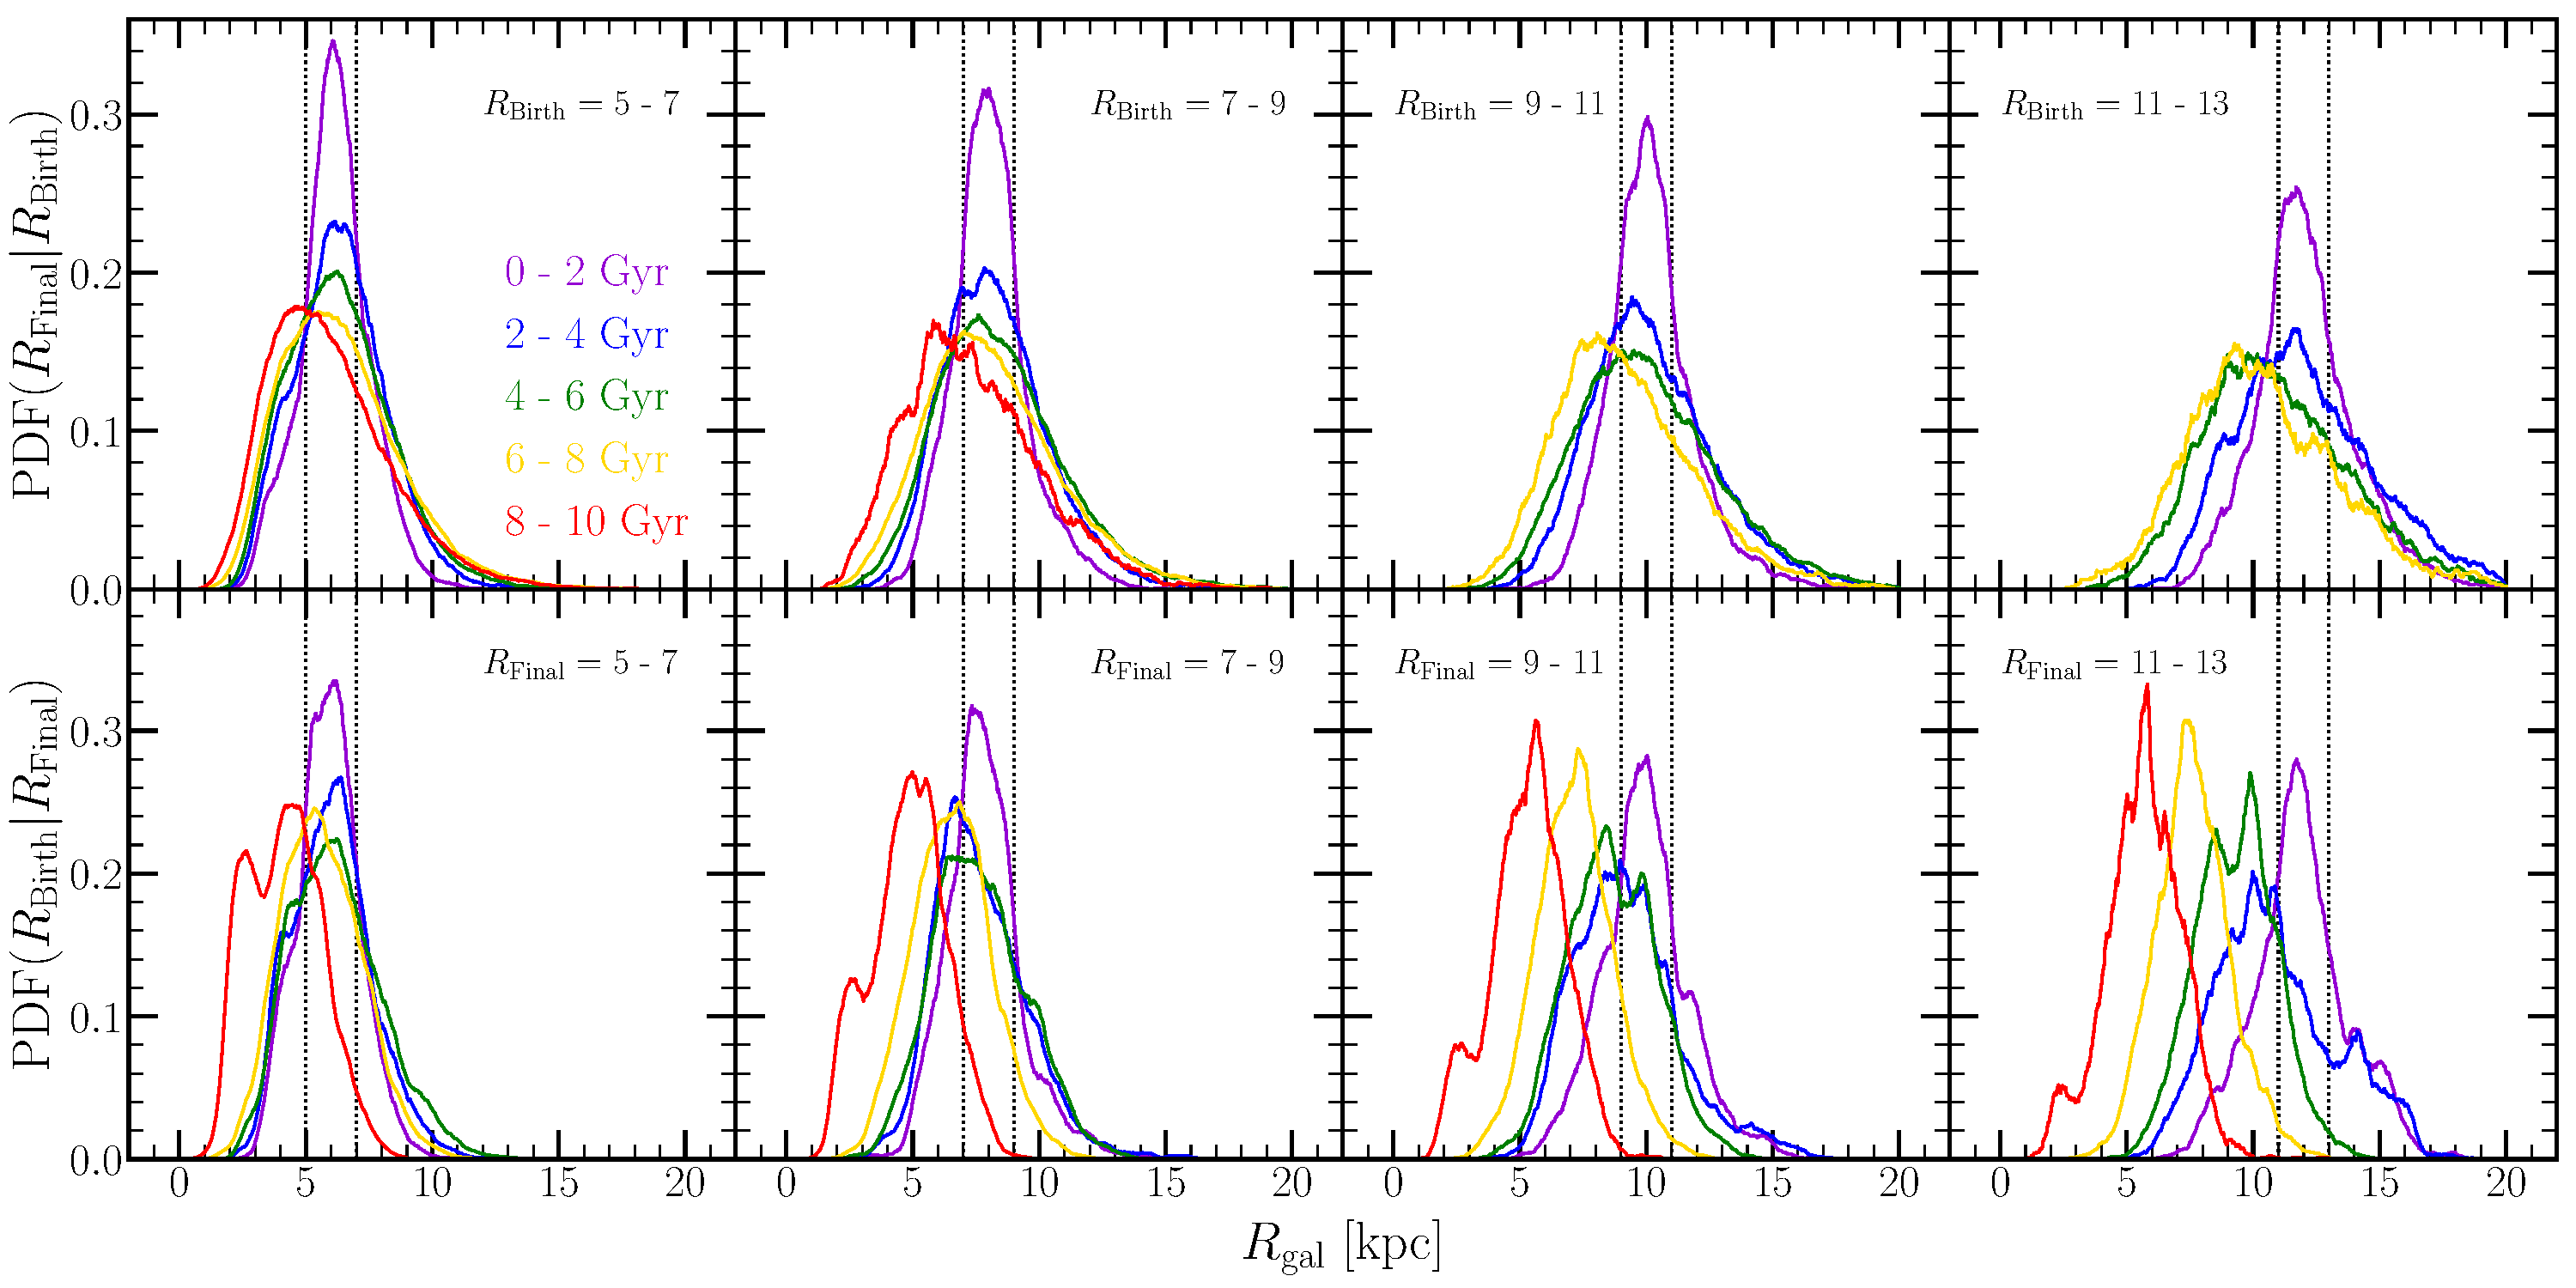
\includegraphics[scale = 0.32]{decomposition.pdf} 
\caption{Radial distributions of our sample of star particles from 
\texttt{h277}. In the top row, we show distributions of~\textit{final} radius 
in bins of birth radius and age, and in the bottom row, we show distributions 
of~\textit{birth} radius in bins of final radius and age. Each bin in 
Galactocentric radius is shown in its own panel, denoted in text at the top of 
each panel and by vertical black dashed lines. We colour-code the distributions 
according to the age of the star particles, denoted by the legend in the upper 
left panel. We smooth all distributions with a box-car width of 0.5 kpc to 
improve visual clarity. We omit the distributions for 8 - 10 Gyr old stars born 
in the 9 - 11 and 11 - 13 kpc bins due to an insufficient number of star 
particles with which to calculate the distribution. } 
\label{fig:h277_decomposition} 
\end{figure*} 

In the top row of Fig.~\ref{fig:h277_decomposition}, we plot the distributions 
of final radius in bins of birth radius and age for our sample of star 
particles. 
Conversely, the bottom row shows distributions of birth radii in bins of final 
radius and age. 
Focusing on the top row of panels, we note that for star particles born at any 
radius and time, the distribution of final radius is still peaked near the 
birth radius, but the peak moves slightly inward with increasing age. 
The tails of the distributions toward larger~$\rgal$ are nearly 
age-independent, while the tails toward smaller~$\rgal$ are not. 
This suggests that radial migration inward and outward occur on different 
timescales in~\texttt{h277}, specifically that inward migration is slower than 
outward migration. 
By extension, this suggests that the two may be tied to different physical 
processes. 
Alternatively, it may simply be that stars that migrate to the outer Galaxy are 
no longer subject to strong dynamical perturbations while stars that move 
inward can still experience strong orbital disturbances. 
\par 
Focusing on the bottom row of panels in Fig.~\ref{fig:h277_decomposition}, we 
note that the modes of the birth radius distributions show a much stronger 
dependence on age than the modes of the final radius distributions. 
At any Galactocentric radius at the present day, the youngest stars are 
overwhelmingly born at comparable radii, while the oldest stars are 
overwhelmingly born at smaller radii. 
This trend is most noticeable at large~$\rgal$. 
The differences between the final radius and birth radius distributions can be 
understood by considering the radial gradient of stellar surface density: there 
are more stars at small radius to move outward than vice versa, so roughly 
symmetric evolution of~$R_\text{final}$ produces strongly asymmetric evolution 
of~$R_\text{birth}$. 
\par 
Taking~$\left|\Delta \rgal\right| \geq$~500 pc 
between birth and final radii as the criterion for migration inward or outward, 
we find as global percentages in our sample that 27\% of star particles 
migrated inward, 29\% migrated outward, and the remaining 44\% stayed near 
their birth radius. 
As one can see from the top panels of Fig.~\ref{fig:h277_decomposition}, a 
large fraction of migration away from birth radius has already occurred by the 
time stars are~$\sim$2 Gyr old. 
If the SN Ia delay-time distribution (DTD) is a~$t^{-1.1} \approx t^{-1}$ 
power-law as suggested by observational results~\citep[e.g.][]{Maoz2012, 
Maoz2017}, then we expect similar numbers of SN Ia events to occur with delay 
times between 0.1 - 1 Gyr and 1 - 10 Gyr. 
With an extended DTD and the timescales for migration implied by 
Fig.~\ref{fig:h277_decomposition}, SN Ia progenitors can migrate significant 
distances before exploding. 
This effect has largely been neglected by GCE studies to date on the grounds 
that radial migration is a slow process, and thus the majority of 
nucleosynthesis should occur near a star's birth radius (e.g. as assumed in 
\citealp{Minchev2013}, and the application of the~\citealp*{Weinberg2017} 
analytic models in~\citealp{Feuillet2018}). 
However, we show below that radial migration within the timescale of the SN Ia 
DTD can have an important impact on some aspects of chemical evolution. 

% \begin{table} 
% % \color{red} 
% \caption{
% For a given quantity in the model, this table summarizes whether it is 
% adopted from~\hsim~or if it is specified as a model parameter. 
% } 
% \begin{tabularx}{\columnwidth}{l @{\extracolsep{\fill}} r} 
% % \resizebox{\columnwidth}{!}{ 
% % \begin{tabular}{l r} 
% \hline 
% \hline 
% Quantity & Source 
% \\ 
% \hline 
% Birth orbital radius of a stellar population & Model 
% \\ 
% Change in orbital radius of a stellar population & \hsim 
% \\ 
% Time-dependence of the change in orbital radius & Model 
% \\ 
% Present-day midplane distance of a stellar population (\absz) & \hsim 
% \\ 
% Star Formation History & Model 
% \\ 
% Nucleosynthetic Yields & Model 
% \\ 
% Outflows from the ISM & Model 
% \\ 
% Star Formation Law & Model 
% \\ 
% Surface Density Gradient & Model 
% \\ 
% \hline 
% \end{tabularx} 
% % } 
% % \label{tab:params} 
% \label{tab:which} 
% \end{table} 

\subsection{Radial Migration} 
\label{sec:methods:migration} 
As in previous studies~\citep[e.g.][]{Matteucci1989, Schoenrich2009a, 
Minchev2013, Sharma2020}, in this paper we model the Milky Way as a series of 
concentric rings\footnote{
	For clarity, we use the term ``ring'' to refer to a computational zone of 
	our calculation (100 pc in radial range) and the term ``annulus'' to refer 
	to a larger radial range (typically 2 kpc). 
} with a uniform width~$\delta \rgal$. 
To run numerical simulations of these models, we develop and make use 
of~\vice's~\texttt{milkyway} object, designed specifically for such an 
approach. 
The~\texttt{milkyway} object is a subclass of a more general object named 
\texttt{multizone}; at its core a~\texttt{multizone} object is an array of 
\texttt{singlezone} objects, which are designed to handle one-zone models of 
GCE and were the focus of~\citet{Johnson2020},~\vice's initial release paper. 
The~\texttt{multizone} object affords users full control over which zone any 
individual stellar population is in at all timesteps following its formation as 
well as the ability to move gas between any two zones with any time dependence. 
In principle this should allow for arbitrarily complex zone configurations and 
migration prescriptions. 
The~\texttt{milkyway} object is a user-friendly extension of the 
\texttt{multizone} base class, which enforces an annular zone configuration as 
we take here. 
As defaults, it adopts the stellar migration model detailed in this section, 
our star formation law discussed in~\S~\ref{sec:methods:sfe}, and the scaling 
of the outflow mass loading factor~$\eta$ with radius~\rgal~parameterized 
in~\S~\ref{sec:methods:outflows}. 
\par 
As in hydrodynamical simulations, star particles in~\vice~are stand-ins for 
entire stellar populations. 
They are said to be in a given zone if their radius is between the inner and 
outer edges of the ring. 
At all times, their nucleosynthetic products and returned envelopes are placed 
in the ISM of the ring that they are in~\textit{at that time}. 
\vice~forms a fixed number of stellar populations per zone per timestep, and it 
allows their masses to vary to account for variations in the SFR. 
The total mass of stars formed in a given zone and timestep is divided evenly 
among the corresponding stellar populations, which can then experience 
different stellar migration histories. 
\par 
The final radius of a stellar population is then determined based on the birth 
and final radii of star particles in the hydrodynamical simulation. 
Describing the Galaxy as a series of concentric rings,~\vice's~
\texttt{milkyway} object assumes stellar populations are born at the centres of 
each ring. 
For a stellar population born at a time~$T$ and Galactocentric radius 
$\rgal$, it first searches for star particles from~\texttt{h277} that 
formed at~$T \pm$~250 Myr and~$\rgal \pm$~250 pc. 
It then randomly selects a star particle from this subsample to act as an 
\textit{analogue}. 
This stellar population then adopts the {\color{red} present day midplane 
distance~$z$ and the} change in orbital radius 
$\Delta \rgal$ of its analogue, and moves from its birth radius to the 
implied final radius at~$T$ = 13.2 Gyr with an assumed time dependence (see 
below). 
If no candidate analogues are found,~\vice~widens the search to~$T \pm$~500 Myr 
and~$\rgal \pm$~500 pc. 
If still no analogue is found, then it finds the star particle with the 
smallest difference in birth radius still within a birth time of $T \pm$~500 
Myr, and assigns it as the analogue. 
{\color{red} 
Because we remove bulge, pseudobulge, and halo star particles from our sample 
(see discussion in~\S~\ref{sec:methods:h277}), every assigned analogue is a 
star particle with disc-like kinematics. 
Since~\hsim~has a similar final disc scale length as the Milky 
Way~\citep{Bird2021}, we do not normalize radii by this quantity prior to 
conducting the analogue search. 
When an~\hsim~star particle is assigned as an analogue, it is~\textit{not} 
thrown out of the sample of candidate analogues, in theory allowing a star 
particle to act as an analogue for multiple stellar populations. Because these 
populations will have similar~$R_\text{form}$~and~$T_\text{form}$, they will 
have similar but not identical abundances. 
}
\par 
While this prescription allows stellar populations to be assigned analogues 
with significantly different birth radii, this is only an issue for small~$T$ 
and large~$\rgal$ where {\color{red} only a small fraction of~\hsim's star 
particles reside,} 
% there are few star particles from~\hsim, 
and where few stars form in nature anyway due to the inside-out growth of 
galaxies~\citep[e.g.][]{Bird2013}. 
{\color{red} 
In practice, we find that our sample of star particles is sufficiently large 
such that our model is still able to assign the vast majority of stellar 
populations born at large~\rgal~($\gtrsim$10 kpc) and small~$T$ 
(age~$\gtrsim$10 Gyr) an analogue which formed within~$\sim$2 kpc of its birth 
radius. 
Although the models we present in this paper do impose a small but non-zero 
level of star formation at early times and large radii (see Fig.~\ref{fig:evol} 
and the associated discussion in~\S~\ref{sec:methods:sfhs}), this ensures that 
those stellar populations inherit plausible dynamics from the~\hsim~star 
particles. 
}
Furthermore, due to the similarity of the histograms in the top row of 
Fig.~\ref{fig:h277_decomposition}, we expect taking~$\Delta \rgal$ from 
a star particle that formed at a similar time but different birth radius in 
these instances to be accurate enough for our purposes. 
{\color{red}
In exploratory work for this paper, we also considered a migration model in 
which stellar populations remain at their birth radius if no analogue born 
within~$\rgal~\pm$~500 pc and~$T~\pm$~500 Myr is found. 
We find similar results in this case, suggesting that our qualitative 
conclusions are largely unaffected by the fine details of the dynamical 
history. 
}
% When an~\hsim~star particle is assigned as an analogue, it is~\textit{not} 
% thrown out of the sample of candidate analogues, in theory allowing a star 
% particle to act as an analogue for multiple stellar populations. Because these 
% populations will have similar~$R_\text{form}$~and~$T_\text{form}$, they will 
% have similar but not identical abundances. 

% fig 2 
\begin{figure} 
\centering 
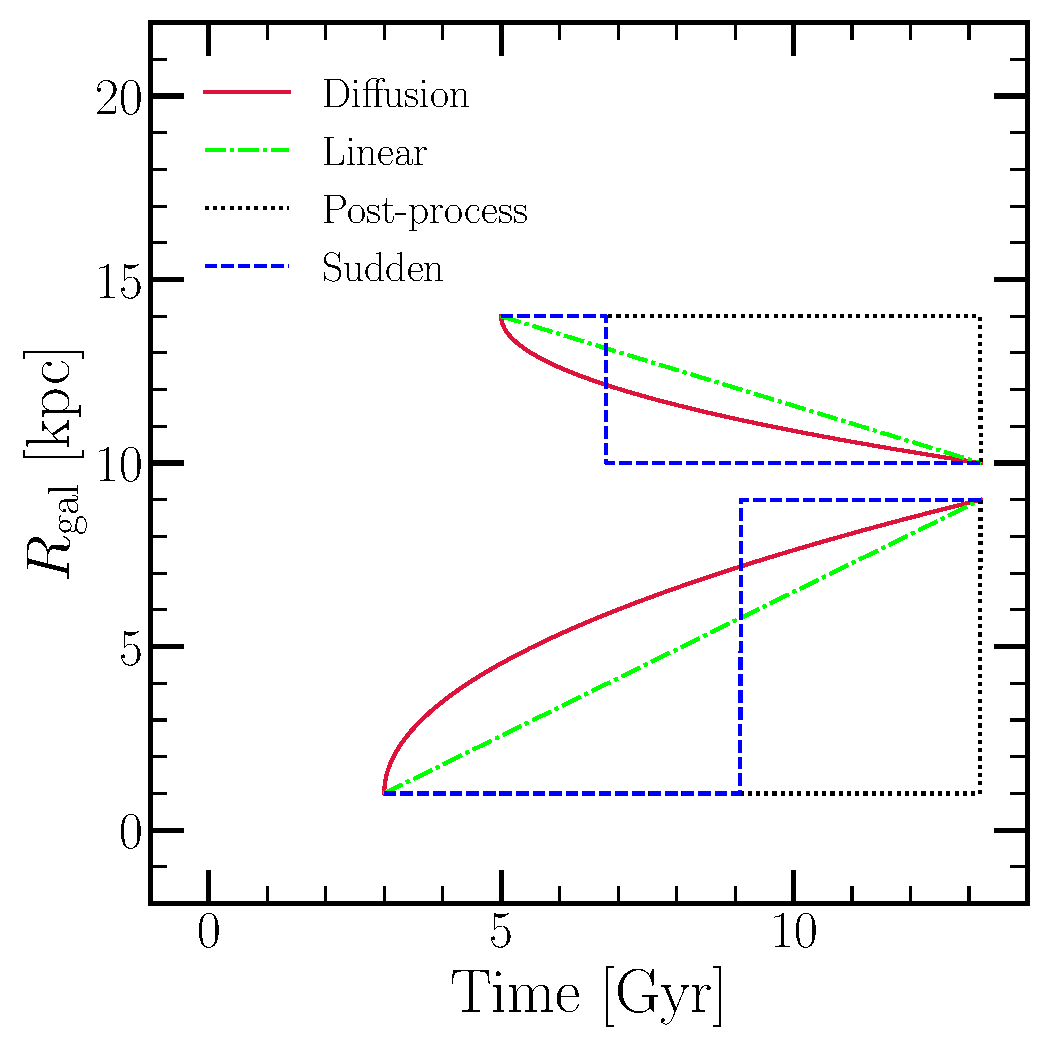
\includegraphics[scale = 0.45]{migration.pdf} 
\caption{A diagram illustrating how Galactocentric radius changes with time for 
two stellar populations under our migration schema: diffusion (crimson, solid), 
linear (lime, dot-dashed), post-process (black, dotted), and sudden (blue, 
dashed). Here the initial and final radii and birth times are chosen at random 
for illustrative purposes. With the initial and final Galactocentric radii of 
a stellar population, its birth time, and one of these assumptions regarding 
the time-dependence of radial migration, the Galactocentric radius at all times 
is known. Diffusion is our default model. } 
\label{fig:migration_schema} 
\end{figure} 

We neglect radial gas flows in the present paper~\citep{Bilitewski2012, 
Lacey1985}, instead focusing our comparisons on the time-dependence with which 
stars migrate. 
We consider four models describing the evolution between a star particle's 
birth and final radius: 
\begin{itemize} 
	\item \textbf{Post-Processing}: Stars stay where they are born until the 
	final timestep, at which point they instantly migrate to their final 
	radius. 
	This retains the assumption that stars do not contribute to nucleosynthesis 
	beyond their birth radius as employed in previous studies 
	\citep[e.g.][]{Minchev2013}. 
	In this scenario, the ISM of each ring is treated as a one-zone model 
	independent of all other zones. We illustrate this case with a black dotted 
	line in Fig.~\ref{fig:migration_schema}. 

	\item \textbf{Sudden}: A random number is drawn from a uniform distribution 
	between a stellar population's time of birth and the present day. 
	That time is taken to be the time of instantaneous migration to the 
	present-day annulus. 
	This emulates a scenario in which a single dynamical interaction rapidly 
	changes a star's orbital radius, and it can be thought of mathematically as 
	a generalization of the post-processing scenario. 
	We illustrate this case with a blue dashed line in 
	Fig.~\ref{fig:migration_schema}. 

	\item \textbf{Diffusion}: Stars move to their final radii in a continuous, 
	time-dependent manner, with displacement~$\propto \sqrt{\text{age}}$. 
	This scenario corresponds to diffusion of angular momentum by a random 
	walk, similar to the assumption used by~\citet{Frankel2018, Frankel2020}. 
	We illustrate this case with a red solid line in 
	Fig.~\ref{fig:migration_schema}. 

	\item \textbf{Linear}: A simple variation of the diffusion model in which 
	the migration to the final radius scales linearly with age rather than with 
	$\sqrt{\text{age}}$. We illustrate this case with a green dot-dashed line 
	in Fig.~\ref{fig:migration_schema}. 
\end{itemize} 
The diffusion model has the clearest physical motivation, and it is our default 
assumption used in all cases unless otherwise noted. 
The other models provide illustrative contrasts and allow us to investigate our 
model's sensitivity to the details of radial migration. 
We do not distinguish between ``blurring'' and ``churning'' 
\citep{Schoenrich2009a}, terms frequenly used to refer to a star's epicyclic 
motions and changes in the guiding centre of its orbit, respectively. 
% We do not distinguish between ``blurring'' and ``churning'', terms frequently 
% used to refer to a star's epicyclic motions and changes in the guiding centre 
% of its orbit~\citep[e.g.][]{Sellwood2002, Schoenrich2009a}. 
Both effects, induced by a wide variety of underlying causes such as molecular 
cloud scattering~\citep{Mihalas1981, Jenkins1990, Jenkins1992}, orbital 
resonances with spiral arms or bars~\citep{Sellwood2002, Minchev2011}, and 
satellite perturbations~\citep{Bird2012}, are present in the~\hsim~simulation. 
\par 
Our GCE model assumes that the star-forming ISM is vertically and azimuthally 
mixed within each radial annulus. 
The abundances assigned to a stellar population depend on its birth radius and 
time, but they do not depend on its distance from the plane. 
Nonetheless, as shown below, the abundance patterns of our simulation exhibit 
clear vertical gradients because older stellar populations have thicker 
vertical distributions~\citep{Bird2021}. 
Radial migration is also coupled to vertical dynamics in complex ways 
\citep{Solway2012, Minchev2012b}. 
We will see that these effects already suffice to explain many of the observed 
vertical trends of Milky Way disc abundances. 


% \subsection{Nucleosynthetic Yields, Outflows, and Recycling} 
% \label{sec:methods:yields} 
\subsection{Nucleosynthetic Yields} 
\label{sec:methods:yields} 
We focus our analysis on alpha and iron-peak elements, taking oxygen (O) and 
iron (Fe) as the representative cases. 
The dominant enrichment channels of interest in our models are thus CCSN and 
SN Ia~\citep{Johnson2019}. 
We would expect similar results for other alpha (e.g. Ne, Mg, Si) and 
iron-peak elements (e.g., Cr, Ni), with quantitative differences reflective of 
their relative yields. 
Odd-$Z$ iron-peak elements (e.g., V, Mn, Co) could behave somewhat distinctly 
because of metallicity-dependent yields. 
\par 
CCSN enrichment happens immediately following the formation of progenitor stars 
in~\vice. 
This is an adequate approximation, because the lifetimes of massive stars are 
short compared to the relevant timescales for galaxy evolution. 
For the most massive stars, the lifetimes are comparable to the timestep size 
we adopt in our numerical integrations. 
This assumption implies a linear relationship between the CCSN enrichment 
rate and the SFR: 
\begin{equation} 
\dot{M}_x^\text{CC} = y_x^\text{CC}\dot{M}_\star 
\end{equation} 
where~$y_x^\text{CC}$ is the CCSN yield of some element~$x$. Physically, this 
quantity represents the mass of an element~$x$ ejected to the ISM from all 
CCSN events associated with a stellar population in units of the stellar 
population's initial mass. 
For example, if~$y_x^\text{CC} = 0.01$, a hypothetical 100~\msun~stellar 
population would add 1~\msun~of~$x$ to the ISM immediately. 
In this paper, we adopt~$y_\text{O}^\text{CC}$ = 0.015 and 
$y_\text{Fe}^\text{CC}$~= 0.0012 from~\citet{Johnson2020}, who in turn adopt 
these values from~\citet{Weinberg2017}. 
\par 
SN Ia nucleosynthesis products are injected according to a~$t^{-1.1}$ DTD with 
a minimum delay time of~$t_\text{D}$ = 150 Myr. 
This is the default DTD in~\vice, which was also adopted by 
\citet{Johnson2020}, and is suggested by recent observational results comparing 
the cosmic SN Ia rate to the cosmic SFH~\citep{Maoz2012, Maoz2017}. 
In a one-zone model at times~$t > t_\text{D}$, the enrichment rate of some 
element~$x$~can be expressed as the product of some yield~$y_x^\text{Ia}$ and 
the SFH weighted by the DTD: 
\begin{subequations}\begin{align} 
\dot{M}_x^\text{Ia} &= y_x^\text{Ia}\langle\dot{M}_\star\rangle_\text{Ia} \\ 
&= y_x^\text{Ia}\ddfrac{
	\int_0^t \dot{M}_\star(t') R_\text{Ia}(t - t') dt' 
}{
	\int_{t_\text{D}}^{t_\text{max}} R_\text{Ia}(t')dt' 
} 
\label{eq:mdot_ia} 
\end{align}\end{subequations} 
where~$R_\text{Ia}$ is the DTD itself, which has units of~$M_\odot^{-1}$ 
Gyr$^{-1}$. 
Like the CCSN yield,~$y_x^\text{Ia}$ is the mass of some element~$x$ produced 
by SNe Ia over the time interval~$t_\text{D} - t_\text{max}$, in units of the 
stellar population's initial mass. 
It can also be expressed as an integral over the DTD: 
\begin{equation} 
y_x^\text{Ia} = m_x^\text{Ia} \int_{t_\text{D}}^{t_\text{max}} R_\text{Ia}(t') 
dt' = m_x^\text{Ia}\frac{N_\text{Ia}}{M_\star} 
\label{eq:y_x_ia} 
\end{equation} 
where~$m_x^\text{Ia}$ is the average mass of the element~$x$ produced in a 
single SN Ia event and the integral evaluates to the mean number of SN Ia 
events~$N_\text{Ia}$ per mass of stars formed~$M_\star$. 
\vice~forces~$t_\text{max}$~= 15 Gyr always, though provided one is consistent 
with equations~\refp{eq:mdot_ia} and~\refp{eq:y_x_ia}, the results are 
independent of~$t_\text{max}$ because the integrals cancel. 
Extending this formalism to multi-zone models is simple; rather than an 
integral over the star formation history of a given annulus, the rate becomes 
a summation over all stellar populations that are in a given zone at some time: 
\begin{equation} 
\dot{M}_x^\text{Ia} = y_x^\text{Ia} \ddfrac{
	\sum_i M_i R_\text{Ia}(\tau_i) 
}{
	\int_{t_\text{D}}^{t_\text{max}} R_\text{Ia}(t')dt' 
} 
\label{eq:mdot_ia_multizone} 
\end{equation} 
where~$M_i$~and~$\tau_i$~are the mass and age of the~$i$'th stellar population, 
respectively. 
\par 
Initially, we adopted~$y_\text{O}^\text{Ia}$~= 0 and~$y_\text{Fe}^\text{Ia}$~= 
0.0017 from~\citet{Johnson2020}, who in turn adopt these values from 
\citet{Weinberg2017}. 
However, we found that the e-folding timescales of star formation in our models 
are sufficiently long (see discussion in~\S~\ref{sec:methods:sfhs}) that our 
fiducial, inside-out SFH model predicted [O/Fe]~$\approx$~+0.05 for young 
stars. 
We therefore multiply~$y_\text{Fe}^\text{Ia}$~by~$10^{0.1}$, adopting 
$y_\text{Fe}^\text{Ia}$~= 0.00214 so that our fiducial model predicts a 
late-time [O/Fe] ratio in better agreement with observations. 
Changes at this level are within the uncertainties of SN Ia rates and yields, 
so we consider it reasonable to adjust the yields empirically to reproduce 
observed abundances. 
\par 
Our IMF-averaged O and Fe yields are based on a~\citet{Kroupa2001} IMF combined 
with supernova nucleosynthesis models in which most~$M > 8~\msun$ stars explode 
as a CCSN~\citep[e.g.][]{Chieffi2004, Chieffi2013}. 
Recent studies have strongly suggested that many high mass stars instead 
collapse directly to a black hole (see theoretical discussion by, e.g., 
\citealp{Pejcha2015, Sukhbold2016, Ertl2016}, and observational evidence from 
\citealp*{Gerke2015};~\citealp{Adams2017, Basinger2020}). 
Our yields would be lower in a scenario with extensive black hole formation 
and/or a steeper high mass IMF~\citep{Griffith2021b}. 
These effects could also introduce a metallicity dependence if the landscape of 
black hole formation changes with metallicity. 
The strong increase of the specific SN Ia rate seen at low galaxy masses 
\citep{Brown2019} provides circumstantial evidence of a higher~$R_\text{Ia}$ 
normalization at low metallicity; the stellar close binary fraction also 
depends on metallicity (\citealp{Badenes2018};~\citealp*{Moe2019}). 
However, there is presently no solid empirical basis for adopting metallicity 
dependent O and Fe yields over the range relevant to this paper (roughly 
-0.8~$\leq$~\feh~$\leq$~0.4), and some empirical evidence that any metallicity 
trends in this range are weak~\citep{Weinberg2019}. 
\vice~has capabilities to compute IMF-averaged yields for a flexible 
description of the massive star explodability landscape, as described 
by~\citet{Griffith2021b} and the~\vice~documentation, but we do not use this 
methodology here. 
We expect that most of our results would be largely unchanged if we were to 
lower all three yields ($y_\text{O}^\text{CC}$, $y_\text{Fe}^\text{CC}$, 
$y_\text{Fe}^\text{Ia}$) by the same factor and adjust our adopted outflow 
mass loading prescription to compensate (see below). 
\par 
Both AGB star enrichment and the recycling of previously produced metals in 
this paper proceed as they did in~\citet{Johnson2020}, with the caveat that the 
mass is added to the ring that a stellar population is in at a given time, 
which may or may not be the ring it was born in. 
Recycling proceeds according to the~\citet{Kalirai2008} initial-remnant mass 
relation assuming a~\citet{Kroupa2001} IMF and a mass-lifetime relationship of 
$\tau = 1.1\tau_\odot(M/M_\odot)^{-3.5}$, where~$\tau_\odot$~= 10 Gyr is the 
main sequence lifetime of the sun and the factor of 1.1 accounts for the 
post-main sequence lifetime. 
\vice~includes AGB enrichment in all models; here we adopt the net yields 
sampled on a table of stellar initial mass and metallicity from the FRUITY 
database \citep{Cristallo2011}. 
However, the AGB star yields of O and Fe are tiny compared to their 
supernova yields, so they have negligible impact on the results presented in 
this paper. 

\subsection{Outflows} 
\label{sec:methods:outflows} 
\citet{Weinberg2017} demonstrate that, to first order, the nucleosynthetic 
yields of a given element and the strength of outflowing winds determine the 
late-time equilibrium abundance in the ISM, with a secondary dependence on the 
SFH. 
We retain their characterization of outflows here, in terms of a mass-loading 
factor~$\eta$~describing the ratio of the mass outflow to the SFR: 
\begin{equation} 
\eta \equiv \frac{\dot{M}_\text{out}}{\dot{M}_\star}. 
\end{equation} 
We adopt a scaling of~$\eta$~with~$\rgal$~such that the late-time 
equilibrium abundance as a function of radius describes a metallicity 
gradient in agreement with observations. 
For a constant SFR, the equilibrium abundance of an~$\alpha$-element, produced 
by CCSNe with a metallicity-independent yield, is given by 
\begin{equation} 
Z_{\alpha,\text{eq}} = \frac{y_\alpha^\text{CC}}{1 + \eta(\rgal) - r}, 
\end{equation} 
where~$r$~is the recycling parameter ($\approx$0.4 for the sake of this scaling 
with a~\citealp{Kroupa2001} IMF; see discussion in~\S~2.2 
of \citealp{Weinberg2017}). Solving for~$\eta(\rgal)$ yields 
\begin{equation} 
\eta(\rgal) = \frac{y_\alpha^\text{CC}}{Z_{\alpha,\text{eq}}} + r - 1 = 
\frac{y_\alpha^\text{CC}}{Z_{\alpha,\odot}}10^{-\text{mode([$\alpha$/H])}
(\rgal)} + r - 1, 
\end{equation} 
where mode([$\alpha$/H])($\rgal$) denotes the mode of the stellar 
[$\alpha$/H] distribution at a radius~$\rgal$, which we assume to correspond 
to the equilibrium abundance at that radius. 
Recent studies of the disc metallicity gradient with APOGEE find values of 
-0.09 dex/kpc to -0.06 dex/kpc~\citep[e.g.][]{Frinchaboy2013, Hayden2014, 
Weinberg2019}, consistent with earlier studies. 
Here we adopt a slope of -0.08 dex/kpc and set mode([$\alpha$/H]) to be 
$\sim$+0.3 at~$\rgal$ = 4 kpc, producing mode([$\alpha$/H])~$\approx$ 0 at 
$\rgal$ = 7 - 9 kpc. This results in the following form for~$\eta$ as a 
function of Galactocentric radius: 
\begin{equation} 
\eta(\rgal) = \frac{y_\alpha^\text{CC}}{Z_{\alpha,\odot}} 
10^{(0.08\text{ kpc}^{-1})(\rgal - 4\text{ kpc}) - 0.3} + r - 1, 
\label{eq:eta_rgal} 
\end{equation} 
where we adopt our CCSN yield of O for~$y_\alpha^\text{CC}$ and the solar 
photospheric abundance of O of~$Z_{\text{O},\odot}$ = 0.00572 based on 
\citet{Asplund2009}. 
We plot this adopted scaling in the top panel of Fig.~\ref{fig:eta_tau_sfh}, 
highlighting a value of~$\sim$2.15 for the solar circle with a red dotted line. 
In Fig.~\ref{fig:metallicity_gradient} below, we show that our full model 
including a time-dependent SFH and radial migration produces stellar and gas 
phase gradients similar but not identical to those of equation 
\refp{eq:eta_rgal}. 
In Figs.~\ref{fig:mdf_3panel_fe} and~\ref{fig:mdf_3panel_o} below, we show that 
the model achieves qualitative agreement with the metallicity gradient observed 
by APOGEE. 

% fig 3 
\begin{figure} 
\centering 
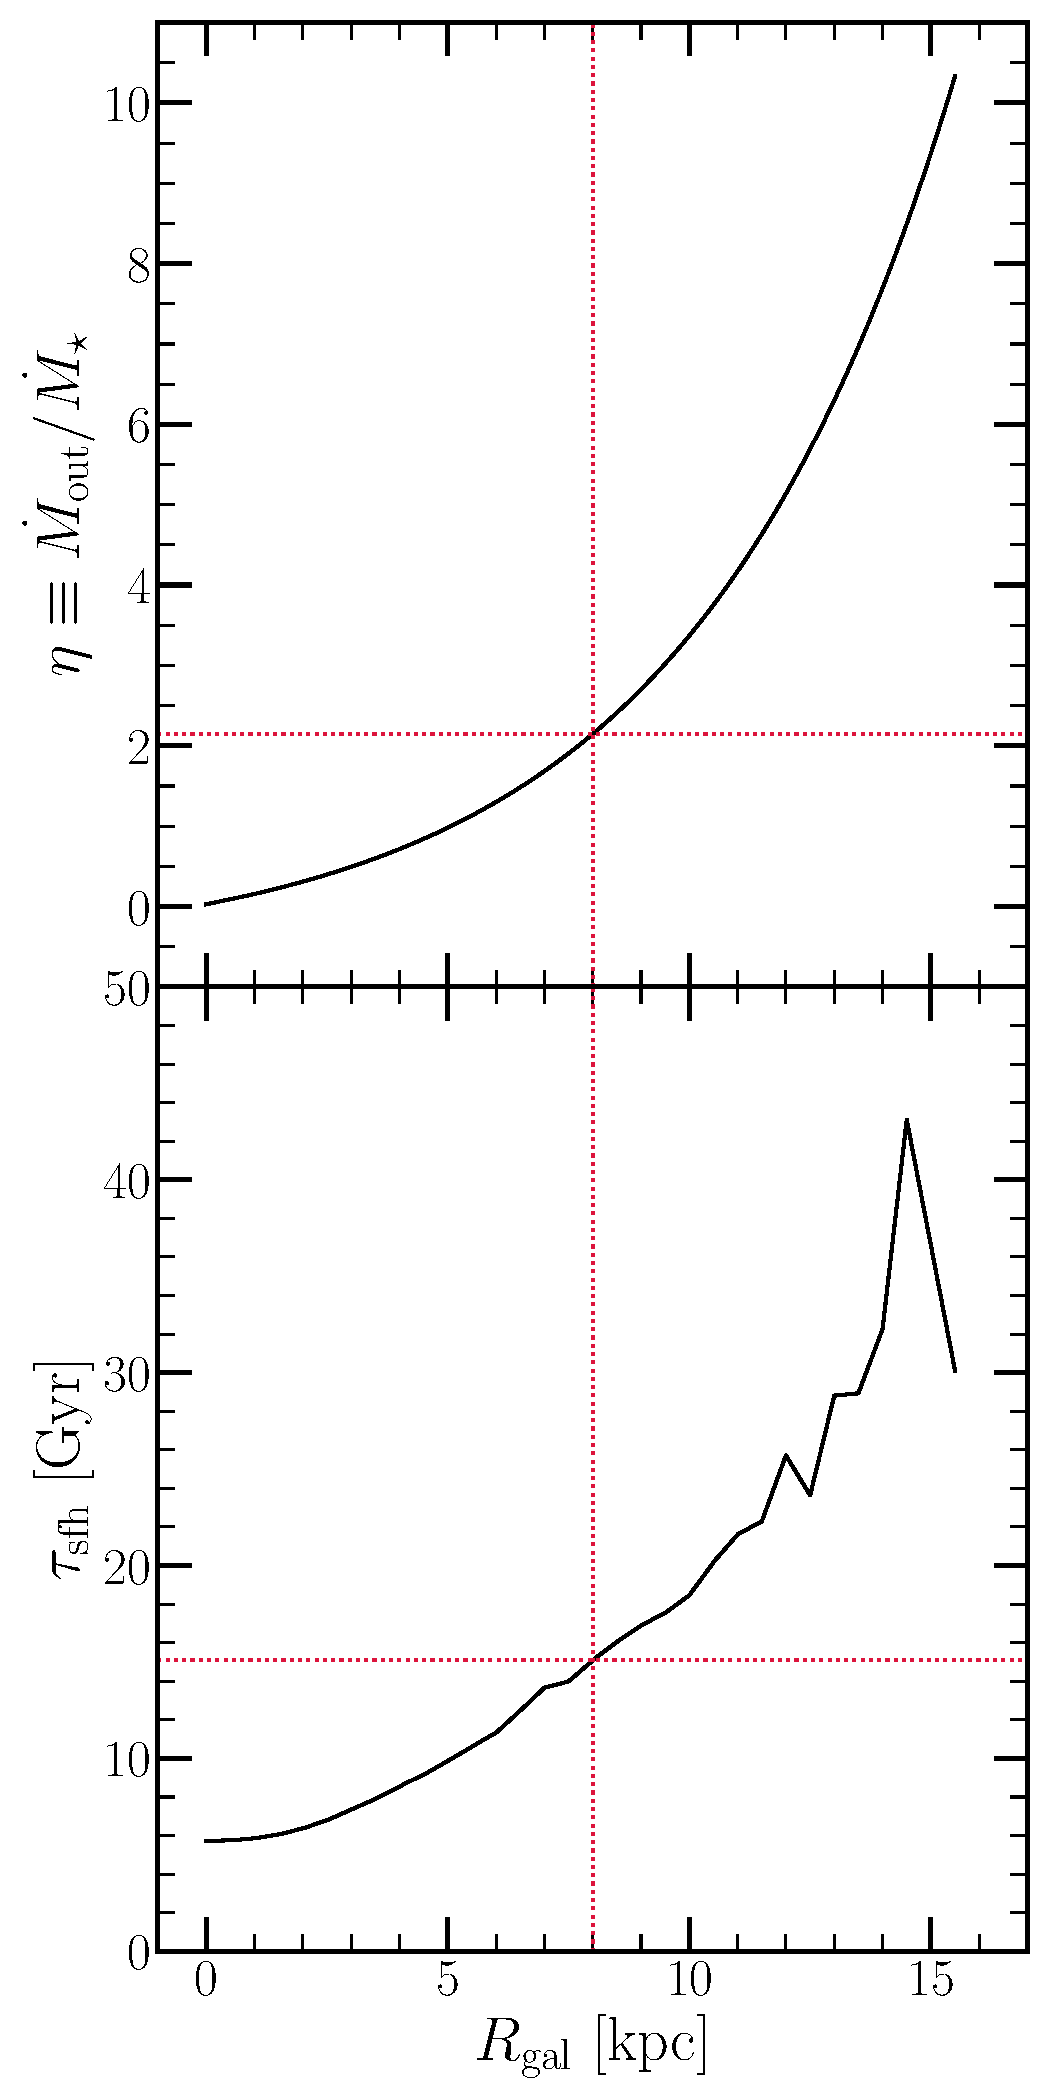
\includegraphics[scale = 0.45]{eta_tau_sfh.pdf} 
\caption{\textbf{Top}: Our implemented scaling of the mass loading factor 
$\eta$~with Galactocentric radius (black) as defined by equation 
\refp{eq:eta_rgal}.~\textbf{Bottom}: The e-folding timescales of the star 
formation histories of our model galaxies (black). These values come from a 
fit to the~$\Sigma_\star$-age relation in bins of~$R/R_\text{e}$~for 
$10^{10.5}$~-~$10^{11}$~\msun~Sa/Sb Hubble type spiral galaxies as reported by 
\citet[][see discussion in~\S~\ref{sec:methods:sfhs}]{Sanchez2020}. The 
horizontal and vertical red dashed lines in both panels highlight a mass 
loading factor of~$\eta \approx$~2.15 and a star formation timescale of 
$\tau_\text{sfh} \approx$~15 Gyr at an assumed radius of the sun of 
$R_\odot$ = 8 kpc. } 
\label{fig:eta_tau_sfh} 
\end{figure} 

\subsection{Star Formation Histories} 
\label{sec:methods:sfhs} 
\vice~computes models in either ``infall'', ``star formation'', or ``gas'' 
mode, referring to which component of the evolutionary history the user has 
specified. 
The starburst models of~\citet{Johnson2020} ran in infall mode, 
meaning that the gas infall rate is specified and the SFR follows from the gas 
surface density and adopted star formation law. 
Here we run~\vice~in star formation mode so that we achieve a specified form of 
the SFHs in our models. 
In Appendix~\ref{sec:normalize_sfh}, we explain how we normalize the parameters 
of our SFHs to produce a realistic model Galaxy at the present day. 
In short, we take a unitless description of the time-dependence of the SFH at a 
given Galactocentric radius, denoted~$f(t|\rgal)$, and a unitless description 
of the present day stellar surface density gradient, denoted~$g(\rgal)$. 
We integrate~$f(t|\rgal)$ with time for each annulus, assuming~$\rgal$ to 
correspond to the centre of the zone, and attach a prefactor to 
$f(t|\rgal)$ in each annulus such that the desired gradient is achieved 
with a total stellar mass similar to the Milky Way. 
This procedure neglects the impact of radial migration, assuming that it does 
not significantly alter the form of~$g(\rgal)$. 
{\color{red} 
We find this to be true for our sample of~\hsim~star particles, and we 
demonstrate that this assumption holds in our chemical evolution models 
in~\S~\ref{sec:methods:surface_density_gradient}, where we also detail our 
adopted form of~$g(\rgal)$. 
}
% We demonstrate that this assumption holds 
% in~\S~\ref{sec:methods:surface_density_gradient}, in which we also detail our 
% adopted form of~$g(\rgal)$. 
The equation derived in Appendix~\ref{sec:normalize_sfh} can be used to 
calculate these prefactors for alternative models of Milky Way-like galaxies. 
\par 
In the present paper, we consider four forms of the SFH, which we dub 
``constant'', ``inside-out'', ``late-burst'', and ``outer-burst''. 
They are defined as follows: 
\begin{itemize} 
	\item \textbf{Constant}: The SFH at a given radius is time-independent, 
	\begin{equation} 
	f_\text{C}(t|\rgal) = 1. 
	\label{eq:constant_sfh} 
	\end{equation} 
	This case is of theoretical interest because it quantifies the effect of 
	stellar migration while removing the impact of a time-dependent SFH. 

	\item \textbf{Inside-Out}: This is our fiducial SFH, 
	\begin{equation} 
	f_\text{IO}(t|\rgal) = (1 - e^{-t / \tau_\text{rise}}) 
	e^{-t / \tau_\text{sfh}}. 
	\label{eq:insideout_sfh} 
	\end{equation} 
	We adopt this mathematical form over the somewhat more common 
	$te^{-t/\tau_\text{sfh}}$ because it allows separate control over the 
	rising and falling phase of the SFH. 
	Equation~\refp{eq:insideout_sfh} has a maximum near~$\tau_\text{rise}$, 
	which in this paper we set to 2 Gyr at all radii. 
	This form produces a peak in star formation at lookback times of~$\sim$11 
	Gyr, roughly corresponding to a redsfhit of~$z \approx$ 2.5. 
	{\color{red} 
	In detail, however, the time of peak star formation increases 
	with~$\tau_\text{sfh}$, which in turn increases with~\rgal~in our models 
	(see discussion below). 
	As a result,~$\dot{\Sigma}_\star$ in the outer disc instead reaches its 
	peak at lookback times of~$\sim$7 - 8 Gyr, qualitatively consistent with 
	the radial growth of the Galaxy~\citep[e.g.][]{Bird2012, Bird2013}. 
	} 
	% We discuss the choice of~$\tau_\text{sfh}$ below. 

	\item \textbf{Late-Burst}: In this model, the inside-out SFH is modified to 
	exhibit a recent, slow ``burst'' in star formation described by a Gaussian 
	in time: 
	\begin{equation} 
	f_\text{LB}(t|\rgal) = f_\text{IO}(t|\rgal) 
	\left(1 + A_be^{-(t - t_b)^2/2\sigma_b^2}\right), 
	\label{eq:lateburst_sfh} 
	\end{equation} 
	where $A_b$ is a dimensionless parameter describing the strength of the 
	starburst,~$t_b$ is the time of the local maximum in the SFH during the 
	burst, and~$\sigma_b$ is the width of the Gaussian describing it. 
	To approximate the findings of~\citet{Mor2019} and~\citet{Isern2019}, we 
	adopt~$A_b$ = 1.5,~$t_b$ = 11.2 Gyr, and~$\sigma_b$ = 1 Gyr, finding 
	that~$A_b$ = 1.5 with a declining~$f_\text{IO}(t|\rgal)$ produces a local 
	maximum SFR that is a factor of~$\sim$2 larger than the preceding local 
	minimum. 

	\item \textbf{Outer-Burst}: A variation of the late-burst model in which 
	only zones at~$\rgal \geq$~6 kpc experience the starburst, with inner 
	regions following the inside-out SFH. 
	Because the empirical evidence for elevated recent star formation comes 
	from local observations, it is useful to investigate the case where it is 
	confined to the outer Galaxy. 
	In their hydrodynamical simulation of a Milky Way-like galaxy, 
	\citet{Vincenzo2020} find that satellite perturbations enhance gas 
	accretion preferentially in the outer regions. 
\end{itemize} 

% fig 4 
\begin{figure*} 
\centering 
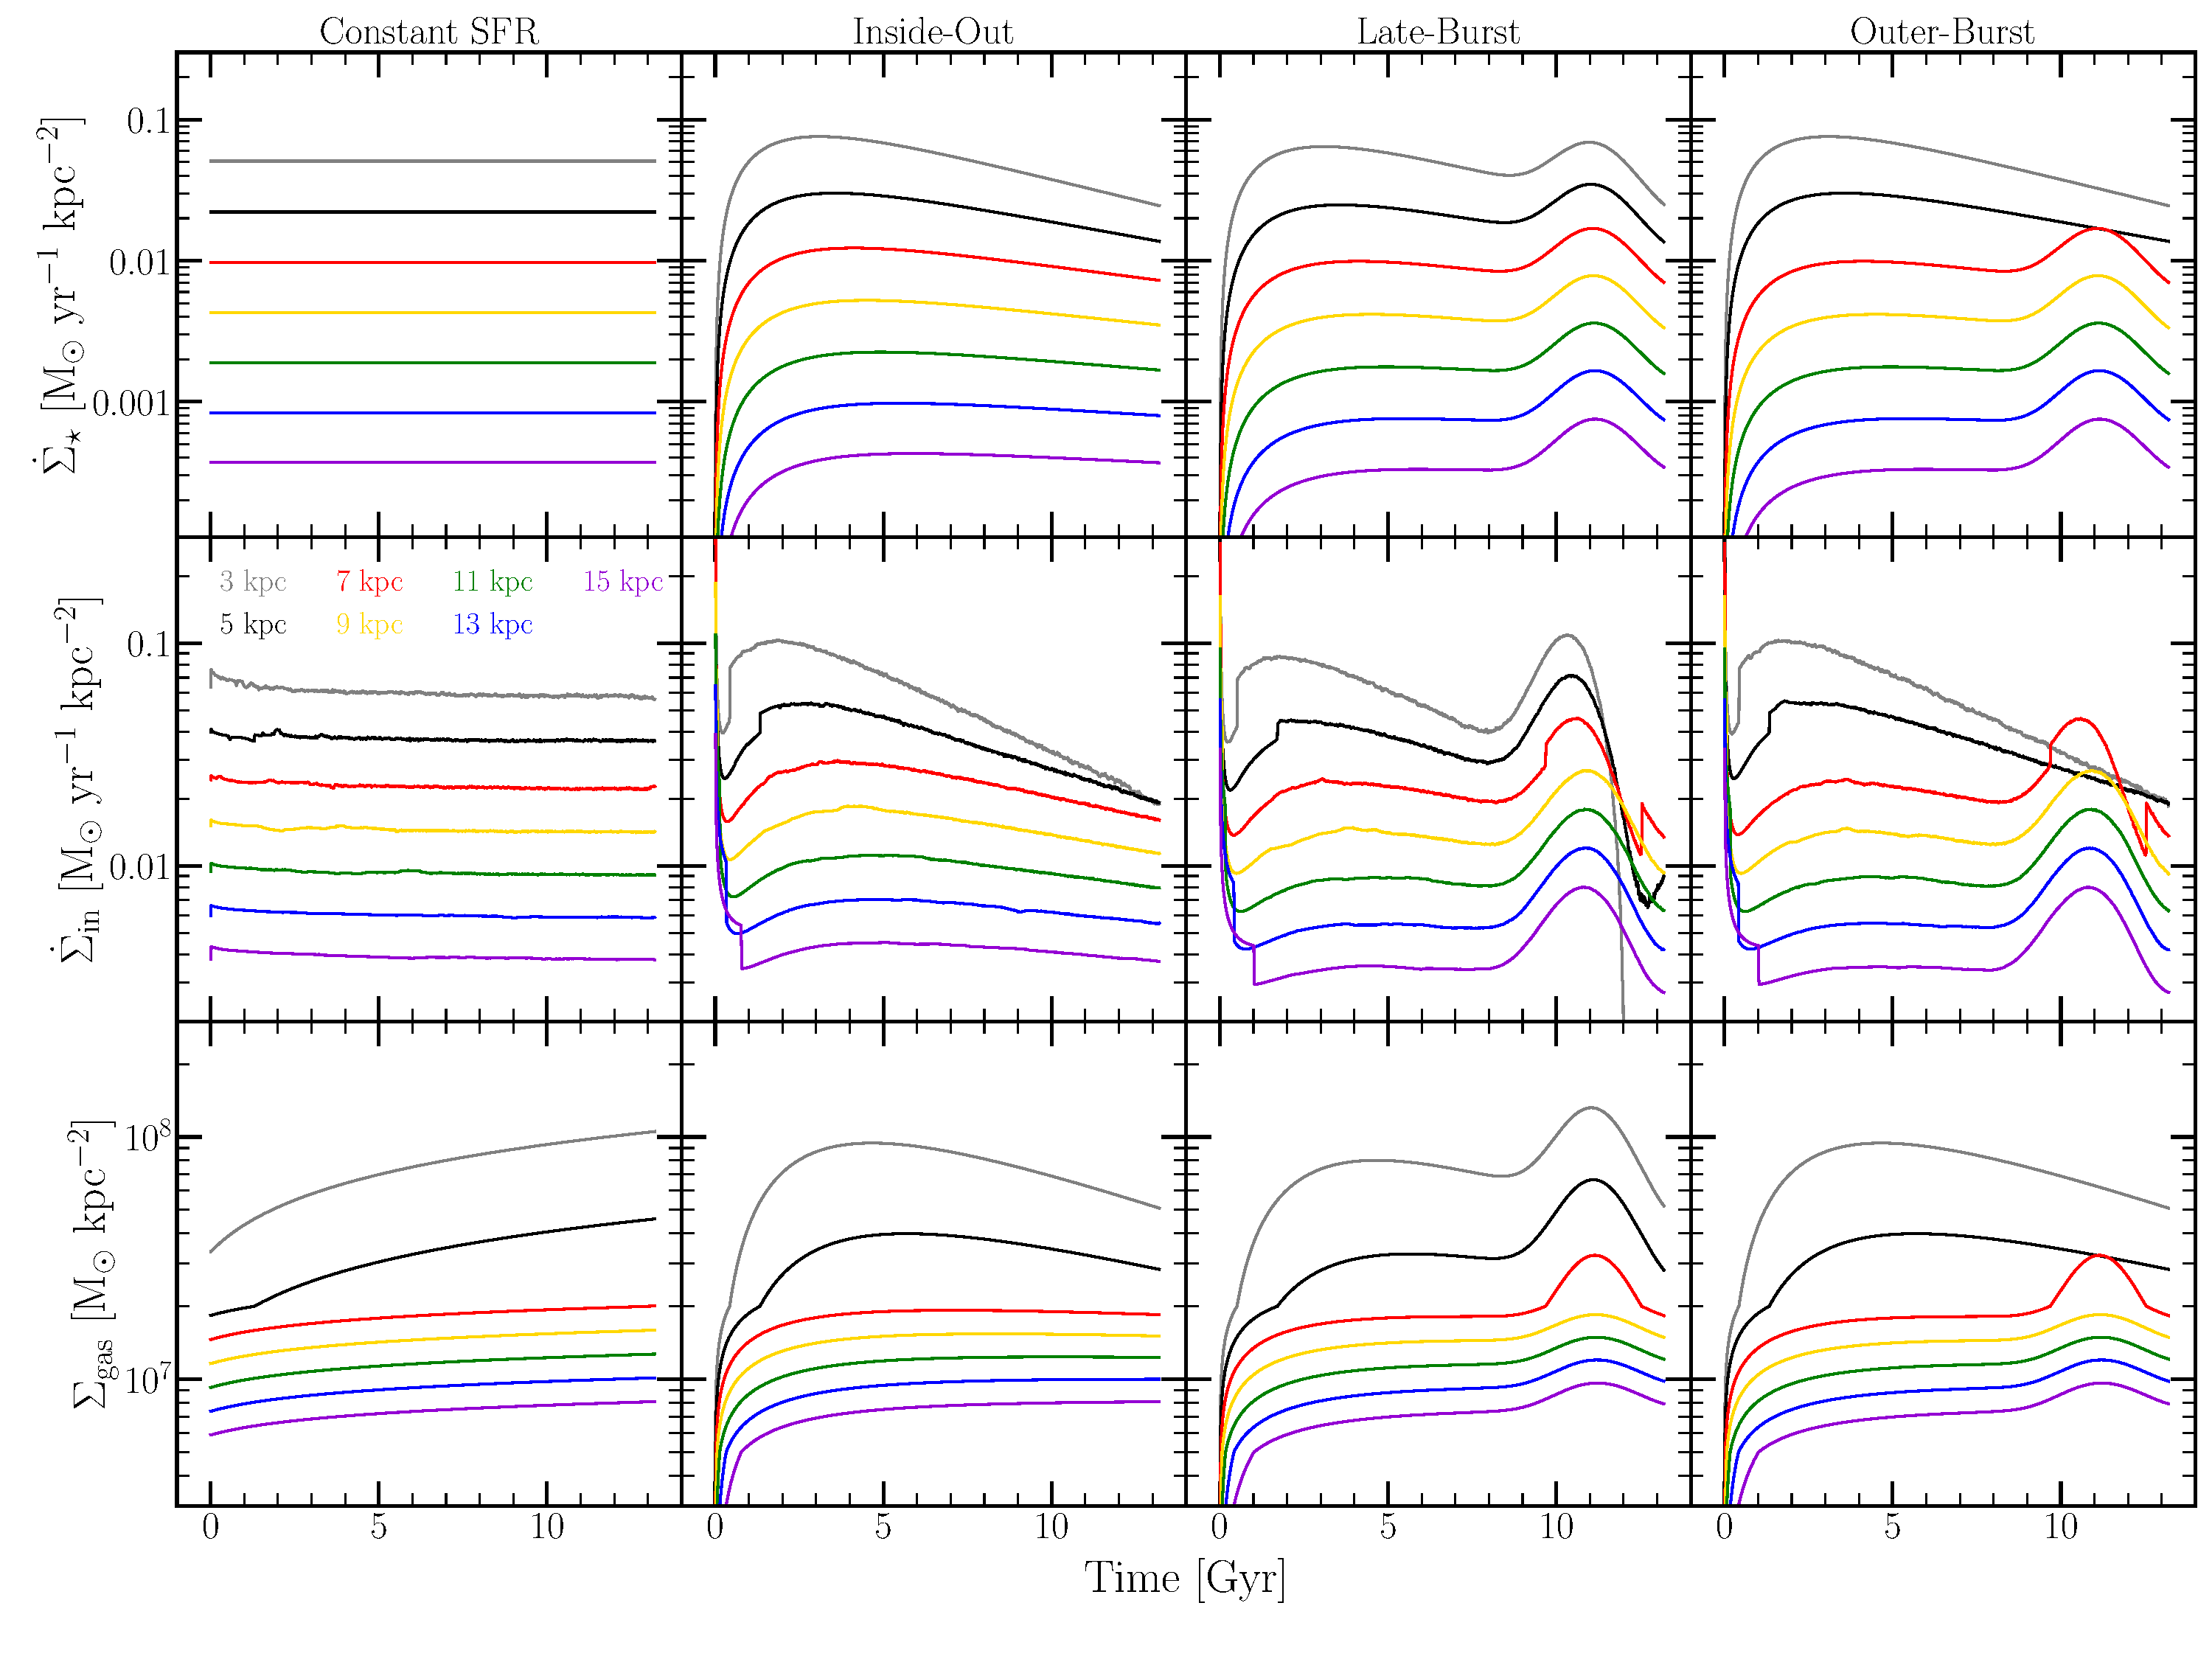
\includegraphics[scale = 0.32]{evol.pdf} 
\caption{The surface densities of star formation~$\dot{\Sigma}_\star$ (top 
row), infall $\dot{\Sigma}_\text{in}$ (middle row), and gas~$\Sigma_\text{g}$ 
(bottom row) as functions of simulation time for our four fiducial SFHs: 
constant (far left), inside-out (left middle), late-burst (right middle), and 
outer-burst (far right). We plot curves for the rings whose inner radii are 
3 kpc (grey), 5 kpc (black), 7 kpc (red), 9 kpc (yellow), 11 kpc (green), 13 
kpc (blue), and 15 kpc (purple) (see equations~\refp{eq:constant_sfh}, 
\refp{eq:insideout_sfh}, and~\refp{eq:lateburst_sfh} for the mathematical 
definition of each SFH). 
}
\label{fig:evol} 
\end{figure*} 

The inside-out model is our fiducial choice, and it is the model shown in 
figures unless otherwise specified. 
The constant SFR model allows us to investigate the impact of migration when 
the time-dependence of the SFH is removed, and the two burst models allow us to 
explore the consequences of elevated recent star formation supported by some 
recent data. 
{\color{red} 
More complex scenarios, such as multiple bursts induced by repeated satellite 
passages~\citep[e.g.][]{Lian2020a, Lian2020b, RuizLara2020, Sysoliatina2021} or 
the onset of star formation occurring later in the outer disc to better capture 
the radial growth of the Galaxy~\citep[e.g.][]{Bird2012, Bird2013}, can be 
explored easily using~\vice, but we do not explore such models here. 
} 
% More complex scenarios with multiple bursts induced by repeated satellite 
% passages~\citep[e.g.][]{Lian2020a, Lian2020b, RuizLara2020, Sysoliatina2021} 
% can be modeled easily in~\vice, but we do not explore them here. 
\par 
We derive the~$\tau_\text{sfh}-\rgal$ relation from the data of 
\citet{Sanchez2020}, who presents the stellar surface density~$\Sigma_\star$ as 
a function of age in bins of~$R/R_\text{e}$ for MaNGA 
galaxies~\citep{Bundy2015}, where $R_\text{e}$ is the half-light radius. 
Here we take the~$M_\star = 10^{10.5} - 10^{11}~\msun$~bin for Sa/Sb spirals 
and simultaneously fit the normalization and e-folding timescale 
$\tau_\text{sfh}$ of our~$f_\text{IO}(t|\rgal)$ form to the data. 
Although the normalization is irrelevant to our models and determined via the 
method outlined in Appendix~\ref{sec:normalize_sfh}, we adopt the resulting 
$\tau_\text{sfh}-\rgal$ relation in our models. 
Our adopted stellar surface density gradient 
(see~\S~\ref{sec:methods:surface_density_gradient}) implies a present-day 
half-mass radius near 4 kpc. 
The findings of~\citet{Garcia-Benito2017} and~\citet{GonzalezDelgado2014} 
suggest that half-light radii are marginally larger than half-mass radii. 
Based on equation (4) of~\citet{GonzalezDelgado2014} relating the two for 
circular apertures, we expect our model Galaxy to have a 
half-light radius near 5 kpc. 
We therefore adopt~$R_\text{e}$ = 5 kpc to convert the 
$\tau_\text{sfh}-\rgal/R_\text{e}$ relation resulting from our fit to the 
\citet{Sanchez2020} data into a~$\tau_\text{sfh}-\rgal$ relation. 
\par 
We illustrate this relationship in the bottom panel of Fig. 
\ref{fig:eta_tau_sfh}. 
The resulting timescales are long, particularly for the outer Galaxy. 
With a red dotted line, we highlight a value of~$\tau_\text{sfh} \approx$~15 
Gyr at an assumed orbital radius of the sun of $R_\odot$ = 8 kpc. 
The long timescales reflect the fact that the 
$\Sigma_\star(\tau_\text{lookback})$ profiles in Fig. 11 of~\citet{Sanchez2020} 
are fairly flat. 
For comparison, we have also considered the assumption that the Galactic SFH 
may have resembled the cosmic SFH by running models with e-folding timescales 
of a~$\sim$few Gyr~\citep[e.g.][]{Madau2014}. 
We find similar results in these cases, suggesting that our qualitative 
conclusions are not sensitive to the exact values of~$\tau_\text{sfh}$. 

We plot the resulting SFHs of our models in the top row of Fig.~\ref{fig:evol} 
for a handful of radii. 
Because of the long~$\tau_\text{sfh}$, the SFR at most radii has fallen only 
modestly from its 2 Gyr peak in the inside-out model. 
{\color{red} 
The gas supply, whose value at all timesteps is known via the star formation 
efficiency timescale~$\tau_\star$ (see~\S~\ref{sec:methods:sfe}), is 
illustrated in the bottom row of Fig.~\ref{fig:evol}. 
}
% At all timesteps, the gas supply is known via the star formation efficiency 
% timescale~$\tau_\star$ (see~\S~\ref{sec:methods:sfe}), which is illustrated in 
% the bottom row of Fig.~\ref{fig:evol}. 
\vice~automatically calculates the implied infall rate by comparing the amount 
of gas lost to outflows and star formation in a given timestep to that which is 
required to sustain the user-specified level of star formation at the next 
timestep; we assume the infalling gas to be of zero metallicity at all times. 
This quantity is shown in the middle row of Fig.~\ref{fig:evol}. 

\subsection{Star Formation Efficiency} 
\label{sec:methods:sfe} 
The term ``star formation efficiency'' (SFE) is somewhat overloaded in the 
literature. 
In the star formation and feedback community, it usually refers to the fraction 
of a molecular cloud's mass that will eventually be converted into stars. 
In the chemical evolution literature, however, it typically refers to the 
inverse timescale relating the SFR within some star forming reservoir to the 
mass of gas in that region: 
$\tau_\star \equiv \Sigma_\text{g}/\dot{\Sigma}_\star$. 
High (Low) values of~$\tau_\star$ indicate slow (fast) conversion of gas and 
thus low (high) SFE; when we refer to SFE here, we mean the definition based on 
this timescale. 
In the star formation and feedback literature,~$\tau_\star$ is sometimes 
referred to as the ``depletion time'', though here we follow the terminology of 
\citet{Weinberg2017} who call it the ``star formation efficiency timescale.'' 
\par 
Based on the findings of~\citet{Kennicutt1998}, it is common practice in the 
chemical evolution literature to adopt a single power-law describing the 
relationship between the surface densities of gas and star formation 
$\Sigma_\text{g}$ and $\dot{\Sigma}_\star$, often referred to as the star 
formation law or the Kennicutt-Schmidt relation: 
\begin{equation} 
\dot{\Sigma}_\star \propto \Sigma_\text{g}^N. 
\end{equation} 
\citet{Kennicutt1998} finds~$N = 1.4 \pm 0.15$ relating the total 
$\dot{\Sigma}_\star$~and~$\Sigma_\text{g}$~within the disc across a sample of 
quiescent spiral galaxies and infrared and circumnuclear starbursts. 
However, recent studies have found evidence that much of the observed scatter 
in this relation is physical in origin~\citep{delosReyes2019} and that there 
are significant breaks in both the power-law index and zero-points 
\citep{Kennicutt2021}. 
Some of the uncertainty surrounding the details of the star formation law is a 
consequence of the ongoing debate about the CO-to-H$_2$ conversion factor 
(\citealp{Kennicutt2012};~\citealp*{Liu2015}). 
Although~\citet{Ellison2021} demonstrate that there are significant 
galaxy-to-galaxy variations in the star formation law,~\citet{delosReyes2019} 
argue that the mean trend is still a reasonable recipe for Galaxy evolution 
models. 
However, for our purposes we also need the dependence of~$\dot{\Sigma}_\star$ 
on~$\Sigma_\text{g}$ within a galaxy. 
% \par 

% fig 5 
\begin{figure} 
\centering 
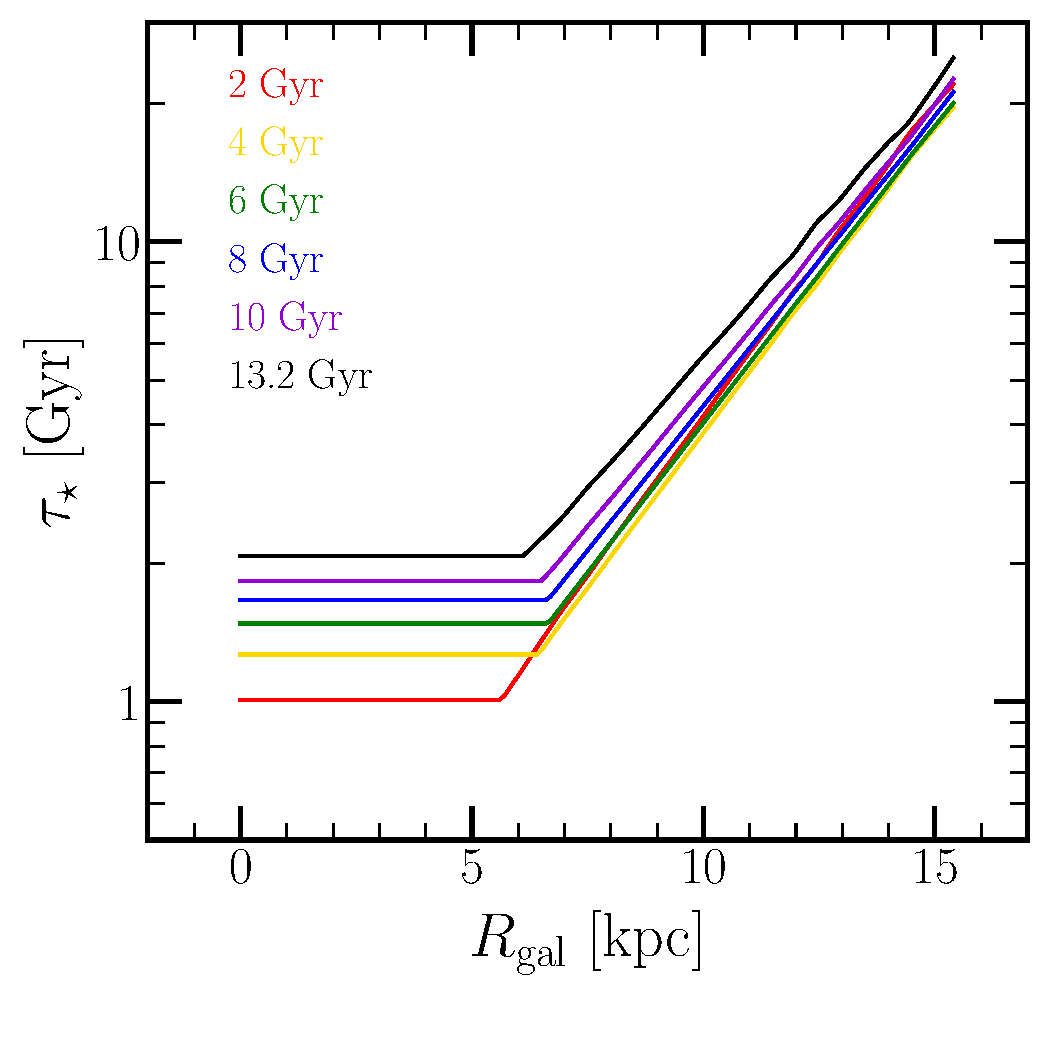
\includegraphics[scale = 0.45]{sfe.pdf} 
\caption{The star formation efficiency timescale~$\tau_\star$ as a function of 
Galactocentric radius at simulation times of 2 Gyr (red), 4 Gyr (yellow), 
6 Gyr (green), 8 Gyr (blue), 10 Gyr (purple), and 13.2 Gyr (the present day, 
black) predicted by our fiducial model. } 
\label{fig:sfe} 
\end{figure} 

\citet{Krumholz2018a} compare theoretically motivated star formation laws to 
the observations of~\citet{Bigiel2010} and~\citet{Leroy2013} (see their Fig. 2). 
We find that the following by-eye fit to the power-law index~$N$~is a 
reasonable description of the aggregate data: 
\begin{equation} 
N = \begin{cases} 
1.0 & (\Sigma_\text{g} \geq \Sigma_{\text{g},2})~, \\ 
3.6 & (\Sigma_{\text{g},1} \leq \Sigma_\text{g} \leq \Sigma_{\text{g},2})~, \\ 
1.7 & (\Sigma_\text{g} \leq \Sigma_{\text{g},1})~, 
\end{cases} 
\label{eq:sf_law_indeces} 
\end{equation} 
where~$\Sigma_{\text{g},1} = 5\times10^6$~\msun~\persqkpc~and 
$\Sigma_{\text{g},2} = 2\times10^7$~\msun~\persqkpc. 
The apparent linearity of the relationship above 
$\sim2\times10^7$~\msun~\persqkpc~suggests that in this regime, star formation 
proceeds at the highest efficiency, and that 
$\tau_\star \equiv \Sigma_\text{g}/\dot{\Sigma}_\star$~= constant. 
The observational results of~\citet{Leroy2013} and~\citet{Kennicutt2021} would 
suggest that these are the surface densities at which the molecular fraction 
$f_\text{mol} = M_{\text{H}_2} / (M_{\text{H}_2} + M_\text{HI}) \approx$~1. 
We therefore adopt the assumption that above 
$\Sigma_\text{g} = 2\times10^7$~\msun~\persqkpc,~$\tau_\star$ reaches its 
minimum value, and increases with decreasing~$f_\text{mol}$. 
We denote this value as~$\tau_\text{mol}$, the value of~$\tau_\star$ for a gas 
reservoir with~$f_\text{mol}$~= 1. 
This identification, combined with our three-component power-law index~$N$ 
results in the following final form for our adopted star formation law: 
\begin{equation} 
\dot{\Sigma}_\star = \begin{cases} 
\Sigma_\text{g} \tau_\text{mol}^{-1} & 
(\Sigma_\text{g} \geq \Sigma_{\text{g},2})~, 
\\ 
\Sigma_\text{g} \tau_\text{mol}^{-1} \left(\frac{
	\Sigma_\text{g}
}{
	\Sigma_{\text{g},2} 
}\right)^{2.6} & 
(\Sigma_{\text{g},1} \leq \Sigma_\text{g} \leq \Sigma_{\text{g},2})~, 
\\ 
\Sigma_\text{g} \tau_\text{mol}^{-1} \left(\frac{
	\Sigma_{\text{g},1} 
}{
	\Sigma_{\text{g},2} 
}\right)^{2.6}\left(\frac{
	\Sigma_\text{g}
}{
	\Sigma_{\text{g},1} 
}\right)^{0.7} & 
(\Sigma_\text{g} \leq \Sigma_{\text{g},1})~. 
\end{cases} 
\label{eq:sf_law} 
\end{equation} 
We choose the power-law indices such that this formalism is consistent 
with equation~\refp{eq:sf_law_indeces}, and prefactors are added to ensure 
piece-wise continuity. 
In implementation,~\vice~requires the~$\tau_\star-\dot{\Sigma}_\star$ relation 
when running in star formation mode and the~$\tau_\star-\Sigma_\text{g}$ 
relation when running in infall and gas modes. 
Both follow algebraically from this relationship given the substitution 
$\tau_\star \equiv \Sigma_\text{g} / \dot{\Sigma}_\star$. 
\par 
Based on the observed Kennicutt-Schmidt relation at different redshifts, 
\citet{Tacconi2018} suggest that~$\tau_\text{mol}$ should scale with redshift 
$z$ and with the deviation from the star forming main sequence~$\delta$MS via 
$\tau_\text{mol} \propto (1 + z)^{-0.6}\delta\text{MS}^{-0.44}$. 
We do not account for the effect of~$\delta$MS in our models, but we do 
incorporate the redshift dependence. 
For redshifts of~$z \lesssim$~3, encompassing most of the timesteps in 
our models, a reasonable approximation to the~$t - z$ relation assuming 
typical~$\Lambda$CDM cosmology is given by: 
\begin{equation} 
\frac{t}{t_0} \approx (1 + z)^{-5/4}, 
\end{equation} 
where~$t_0$ is the present-day age of the universe, and~$t$ is not simulation 
time but the age of the universe. Plugging this relation into the 
\citet{Tacconi2018} scaling yields 
\begin{equation} 
\tau_\text{mol} = \tau_{\text{mol},0}(t/t_0)^{12/25} \approx 
\tau_{\text{mol},0}(t/t_0)^{1/2}, 
\end{equation} 
where~$\tau_{\text{mol},0}$ is simply~$\tau_\text{mol}$ at the present day. We 
generalize this formula to the following form: 
\begin{equation} 
\tau_\text{mol} = \tau_{\text{mol},0}(t/t_0)^\gamma 
\label{eq:tau_mol}
\end{equation} 
In this paper we present models which adopt~$\tau_{\text{mol},0}$ = 2 Gyr 
\citep{Leroy2008, Leroy2013, Tacconi2018} and~$\gamma$ = 1/2 based on this 
argument. 
We have also run simulations witht~$\tau_{\text{mol},0}$ = 1 
Gyr and with~$\gamma$ = 0 (a time-independent~$\tau_\text{mol}$), as well as 
combinations of the two, and found similar results. 
In all timesteps and annnuli,~\vice~infers~$\Sigma_\text{g}$ from 
$\dot{\Sigma}_\star$ given our equations~\refp{eq:sf_law} and~\refp{eq:tau_mol}. 
\par
In Fig.~\ref{fig:sfe}, we plot~$\tau_\star$ as a function of~$\rgal$ at 
six different time stamps predicted by our fiducial, inside-out SFH model. 
At~$\rgal \lesssim$ 6 kpc,~$\tau_\star$ is near~$\tau_\text{mol}$ at all 
times, implying a molecular fraction of unity at these radii. 
Although this prediction is likely unrealistic because 21-cm line observations 
suggest the presence of neutral hydrogen as close to the Galactic centre as 
several hundred pc~\citep{Kalberla2009}, we find in practice that changing our 
assumptions about the star formation law does not impact our conclusions. 
In exploratory work for this paper, we investigated purely linear, purely 
power-law, and broken power-law characterizations, finding similar predictions 
in all cases. 
In general we find that the detailed form of the SFH, and to some extent the 
time-dependence of radial migration, exert much greater power in establishing 
the model predictions than does the star formation law. 
Nonetheless it is an interesting puzzle that a 
$\dot{\Sigma}_\star - \Sigma_\text{g}$ relation informed by the observed 
population-averaged trends and the normalization of SFHs implied by the stellar 
mass of the Milky Way predicts results in tension with the observed HI 
distribution. 
Because the star formation law has minimal impact on our results, we do not 
pursue this question further here. 

\subsection{Surface Density Gradient} 
\label{sec:methods:surface_density_gradient} 

\begin{table*} 
% \color{red} 
\caption{
A summary of our chemical evolution model parameters, their fiducial values, 
and in what section of the text relevant discussion can be found. 
}
\begin{tabularx}{\textwidth}{l @{\extracolsep{\fill}} l l r} 
\hline 
\hline 
Quantity & Section & Description & Fiducial Value(s) 
\\ 
\hline 
\rgal & N/A & Galactocentric Radius & $0 - 20$ kpc 
\\ 
$\delta$\rgal & \ref{sec:methods:summary} & Width of each concentric ring & 
100 pc 
\\ 
$\Delta$\rgal & \ref{sec:methods:migration} & Change in orbital radius due to 
stellar migration; adopted from~\hsim~analogue star particle & N/A 
\\ 
$z$ & \ref{sec:methods:migration} & Present day distance to Galactic midplane; 
adopted from~\hsim~analogue star particle & $-3 - +3$ kpc 
\\ 
$T_\text{max}$ & \ref{sec:methods:h277} & Time interval over which our models 
are integrated & 13.2 Gyr 
\\ 
$\delta T$ & \ref{sec:methods:summary} & Timestep size & 10 Myr 
\\ 
$n$ & \ref{sec:methods:summary} & Number of stellar populations formed per ring 
per timestep & 8 
\\ 
$R_\text{SF}$  & \ref{sec:methods:summary} & Maximum radius of star formation 
(i.e.~$\dot{\Sigma}_\star$ = 0 at~\rgal~>~$R_\text{SF}$) & 15.5 kpc 
\\ 
$\tau_\star$ & \ref{sec:methods:sfe} & The SFE timescale of the ISM: 
$\tau_\star \equiv \Sigma_\text{gas} / \dot{\Sigma}_\star$ & N/A 
\\ 
$\tau_{\text{mol},0}$ & \ref{sec:methods:sfe} & The SFE timescale of molecular 
hydrogen at the present day & 2 Gyr 
\\ 
$\gamma$ & \ref{sec:methods:sfe} & The power-law index describing the 
time-dependence of the molecular hydrogen SFE timescale 
(i.e.~$\tau_\text{mol}\sim t^\gamma$) & 1/2 
\\ 
$\eta$ & \ref{sec:methods:outflows} & The outflow mass-loading factor: 
$\eta \equiv \dot{\Sigma}_\text{out}/\dot{\Sigma}_\star$ (assumed to be 
time-independent) & equation~\refp{eq:eta_rgal} 
\\ 
$y_\text{O}^\text{CC}$ & \ref{sec:methods:yields} & CCSN yield of O & 0.015 
\\ 
$y_\text{Fe}^\text{CC}$ & \ref{sec:methods:yields} & CCSN yield of Fe & 0.0012 
\\ 
$y_\text{O}^\text{Ia}$ & \ref{sec:methods:yields} & SN Ia yield of O & 0 
\\ 
$y_\text{Fe}^\text{Ia}$ & \ref{sec:methods:yields} & SN Ia yield of Fe & 0.00214 
\\ 
$\dot{\Sigma}_\star$ & \ref{sec:methods:sfhs} & Surface density of star 
formation & N/A
\\ 
$f_\text{IO}(t|\rgal)$ & \ref{sec:methods:sfhs} & The time-dependence of the 
star formation history in the inside-out model & 
equation~\refp{eq:insideout_sfh} 
\\ 
$f_\text{LB}(t|\rgal)$ & \ref{sec:methods:sfhs} & The time-dependence of the 
star formation history in the late-burst model & 
equation~\refp{eq:lateburst_sfh} 
\\ 
\hline 
\end{tabularx} 
\label{tab:params} 
\end{table*} 

% As discussed in~\S~\ref{sec:methods:sfhs}, Appendix~\ref{sec:normalize_sfh} 
% presents the recipe by which we select a unitless function describing the 
% stellar surface density gradient~$g(\rgal)$. 
{\color{red} 
As discussed in~\S~\ref{sec:methods:sfhs}, Appendix~\ref{sec:normalize_sfh} 
presents the recipe by which we normalize our star formation histories, a 
necessary component of which is a unitless function describing the stellar 
surface density gradient~$g(\rgal)$. 
}
In setting the normalization, our model ensures that the integral of~$g(\rgal)$ 
over the surface area of the disc predicts a total stellar mass in agreement 
with that observed for the Milky Way. 
For this value, we adopt~$M_\star^\text{MW} = 5.17~\times~10^{10}~\msun$ from 
\citet[][$\pm 1.11\times10^{10}~\msun$]{Licquia2015}. 
This is the total disc mass only; when the bulge is included, the total 
becomes~$(6.08~\pm~1.17)~\times~10^{10}~\msun$. 
Since we are modeling only the disc populations here, we omit the contribution 
from the bulge to the total mass budget. 
% For this value, we adopt 
% $M_\star^\text{MW} = (5.17 \pm 1.11)\times10^{10}$~\msun~\citep{Licquia2015}. 
% This is the total disc mass of the Galaxy;~\citet{Licquia2015} report 
% $(6.08 \pm 1.17)\times10^{10}~\msun$~when the bulge is considered. 
% Since we are modeling only the disc populations here, we omit the contribution 
% the bulge would have to the total mass budget. 
% This is the total stellar mass of the Galaxy, including the bulge; 
% \citet{Licquia2015} report~$(5.17 \pm 1.11)\times10^{10}$~\msun~as the mass of 
% the disc alone. 
% Although we are not modeling the bulge here, our model extends to~$\rgal$ = 0 
% and our sample of candidate analogue star particles from~\hsim includes those 
% with bulge-like kinematics. 
\par 
We adopt a double exponential form for~$g(\rgal)$, describing the thin and 
thick disc components of the Galaxy: 
\begin{equation} 
g(\rgal) = e^{-\rgal/R_t} + \frac{\Sigma_T}{\Sigma_t} 
e^{-\rgal/R_T}~, 
\label{eq:gradient} 
\end{equation} 
where~$R_t$~and~$R_T$~are the scale radii of the thin and thick discs, 
respectively, and~$\Sigma_T/\Sigma_t$~is the ratio of their surface densities 
at~$\rgal$~= 0. 
We adopt~$R_t$~= 2.5 kpc,~$R_T$~= 2.0 kpc, and~$\Sigma_T/\Sigma_t$~= 0.27 based 
on the findings of~\citet{Bland-Hawthorn2016}. 
We plot the single exponential forms of each disc component as dotted black 
lines in Fig.~\ref{fig:surface_density}, with the solid black line denoting the 
sum of the two. 

% fig 6 
\begin{figure} 
\centering 
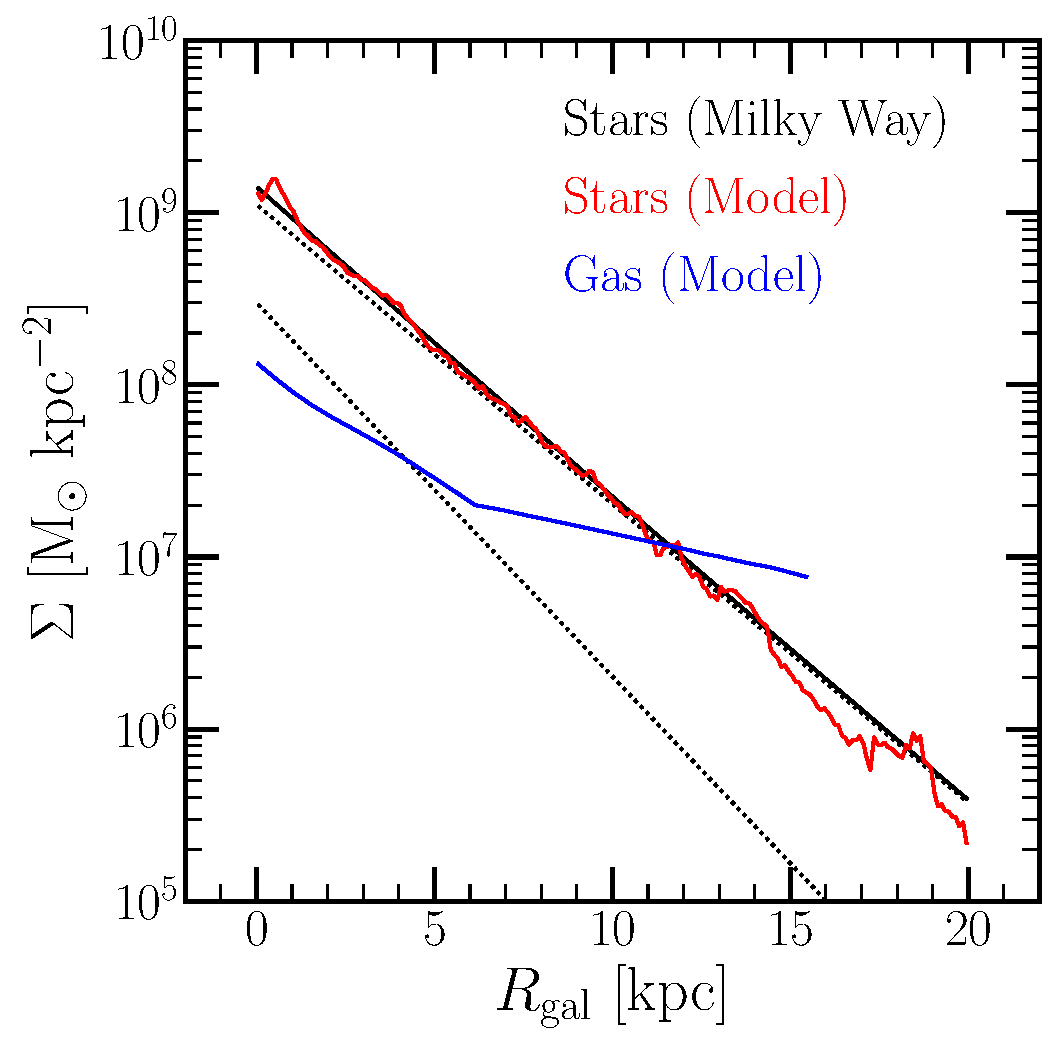
\includegraphics[scale = 0.45]{surface_density_gradient.pdf} 
\caption{The surface density of gas (blue) and stars (red) as predicted by our 
fiducial model. The dotted black lines denote thin and thick disc 
profiles with scale lengths of~$R_t$ = 2.5 kpc and~$R_T$ = 2.0 kpc, 
respectively, with a ratio of~$\Sigma_T/\Sigma_t$ = 0.27 at~\rgal~= 0 (i.e. the 
thin disc profile has the higher normalization). 
The solid black line denotes the sum of the two; this is the stellar surface 
density gradient of the Milky Way as reported by~\citet{Bland-Hawthorn2016}, 
renormalized according to our adopted total stellar mass of 
$(5.17 \pm 1.11)\times10^{10}$~\msun~\citep{Licquia2015}. } 
\label{fig:surface_density} 
\end{figure} 

We plot the resultant surface density gradients from our fiducial, inside-out 
SFH model in Fig.~\ref{fig:surface_density} as well, with red denoting the 
stellar gradient and the gas in blue. 
The stellar gradient very nearly follows our target gradient (equation 
\ref{eq:gradient}) denoted by the solid black line. 
{\color{red} 
Simply introducing scatter around the adopted trend, stellar migration has 
not significantly altered the overall form of the gradient, as we assumed in 
Appendix~\ref{sec:normalize_sfh}; we find this to also be true for our sample 
of star particles from~\hsim. 
}
% Stellar migration has not altered the overall form of the gradient, simply 
% introducing scatter around the adopted trend. 
Although there are slight enhancements at small~$\rgal$ and deficits at large 
$\rgal$, the agreement is excellent in the regions of the Galaxy where the 
gradient is best constrained observationally. 
The~$\rgal$ > 15.5 kpc populations are composed entirely of stars that 
migrated there, since that is the radius at which we shut off star formation. 
The gas gradient shows a break in the scale radius near~$\rgal \approx$ 
6 kpc. This is a consequence of our adopted star formation law; at 
$\Sigma_\text{g} = 2\times10^7$~\msun~\persqkpc~the relation changes from 
linear at higher densities to~$\dot{\Sigma}_\star \sim \Sigma_\text{g}^{3.6}$ 
at lower densities (see discussion in~\S~\ref{sec:methods:sfe}). 
\par 
Although we adopt the~\citet{Licquia2015} disc stellar mass of the Milky Way 
here, we find similar results when taking a value which differs even by an 
order of magnitude. 
If we used a linear star formation law, then our chemical evolution would be 
independent of the mass normalization as it is in corresponding one-zone 
models (\citealp*{Spitoni2017};~\citealp{Weinberg2017, Belfiore2019}). 
The mass normalization enters our calculation because it affects the transition 
between the linear and non-linear regimes of our star formation law 
(equation~\ref{eq:sf_law}), but the impact on abundance evolution is minimal. 

\subsection{Summary} 
\label{sec:methods:summary} 

% fig 7 
\begin{figure*} 
\centering 
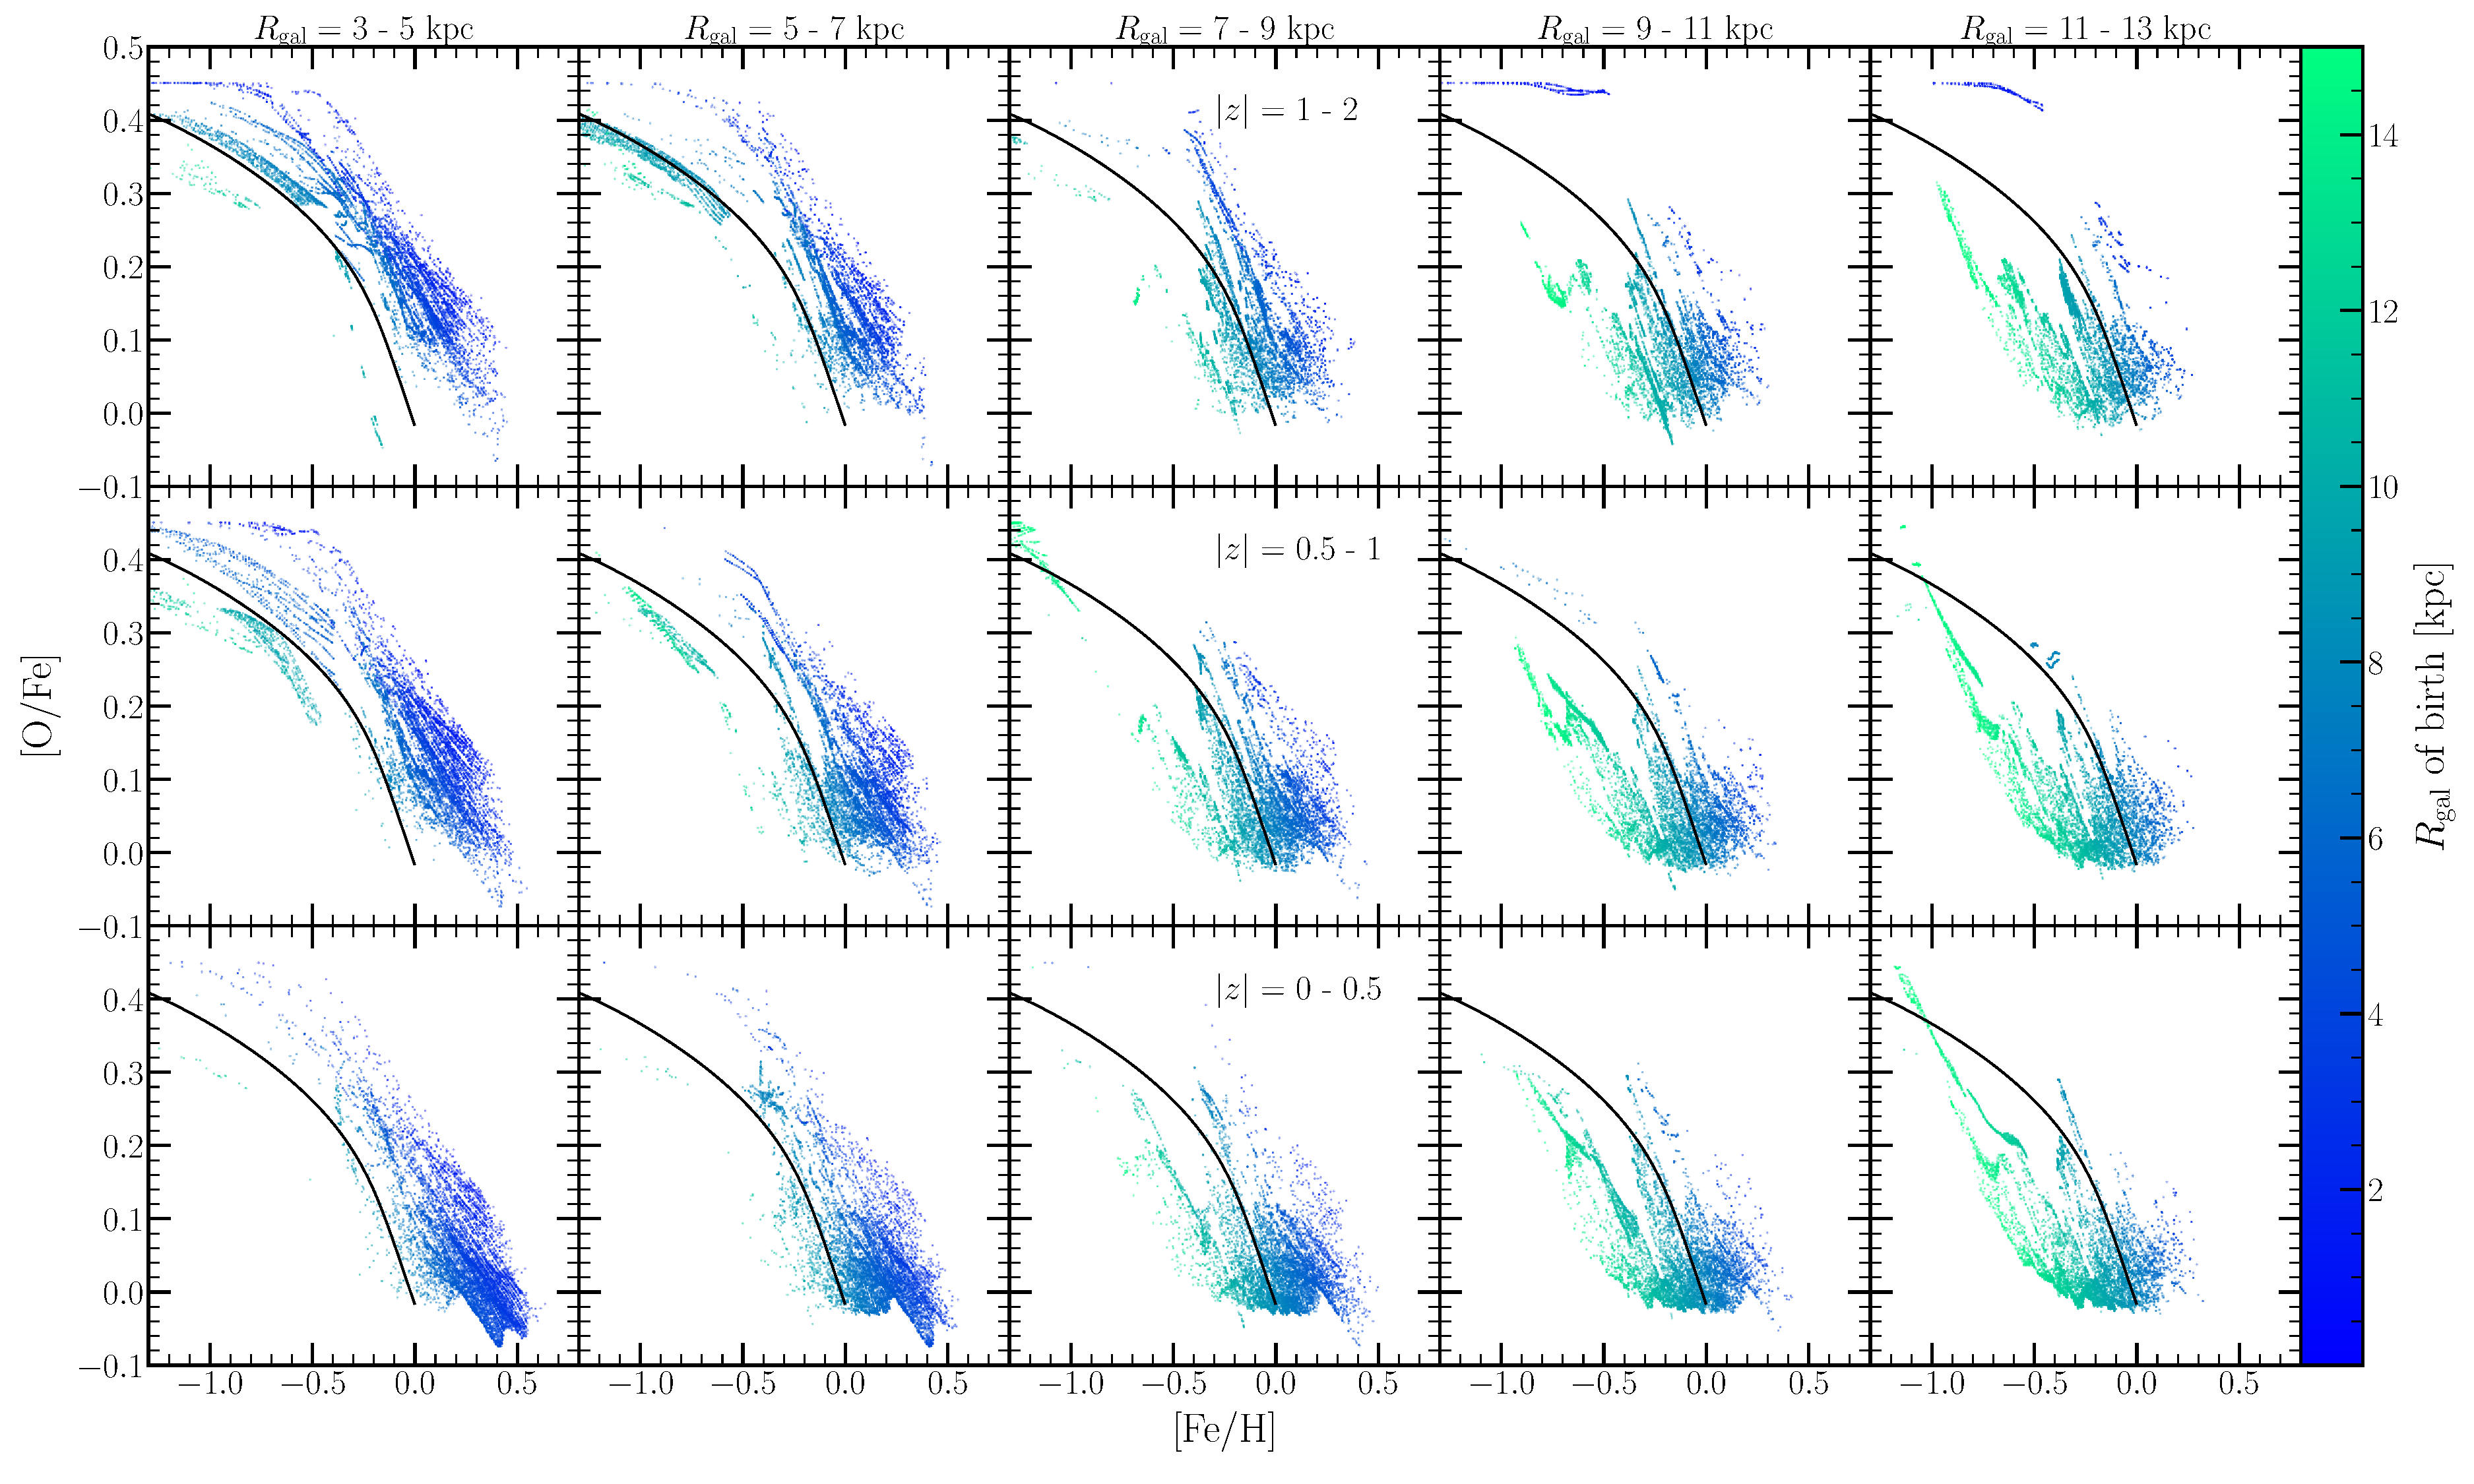
\includegraphics[scale = 0.28]{ofe_feh_densitymap.pdf} 
\caption{[O/Fe]-[Fe/H] diagrams for 15 Galactic regions spanning five bins in 
$R_\text{gal}$ and three in~$\left|z\right|$. Each region has its own panel, 
with radial bins shown in columns denoted at the top, and with bins in 
$\left|z\right|$ shown in rows denoted in text in the middle column. For each 
region, we plot~$N$~= 10,000 points sampled from our simulated stellar 
populations predicted by our fiducial model, where the probability of 
sampling is proportional to the present-day mass of each stellar population. 
In all panels, points are colour-coded according to the Galactocentric radius 
of birth of the stellar population. For reference, we plot in a solid black 
line in all panels the gas-phase [O/Fe]-[Fe/H] track predicted by the same 
SFH in the~$R_\text{gal}$ = 8 kpc annulus, but with the post-processing 
migration model; this curve is the same in all panels. } 
\label{fig:ofe_feh_diagram} 
\end{figure*} 

{\color{red} 
Table~\ref{tab:params} presents a breakdown of our model parameters, their 
values, and references to the sections where relevant discussion can be found. 
}
In summary, our fiducial model has an inside-out SFH with e-folding timescales 
derived from the observations of~\citet[][see discussion 
in~\S~\ref{sec:methods:sfhs}]{Sanchez2020}. 
Radial migration proceeds in a manner in which our model stellar populations 
have a change in radius~$\Delta \rgal$ informed from the~\texttt{h277} 
hydrodynamical simulation~\citep[][see discussion 
in~\S~\ref{sec:methods:h277}]{Christensen2012, Zolotov2012, Loebman2012, 
Loebman2014, Brooks2014}. 
In the baseline model, stars move to their final radius with a 
$\sqrt{\text{age}}$~dependence~\citep[][see discussion in 
\ref{sec:methods:migration}]{Frankel2018,Frankel2020}. 
Using~\vice~to calculate abundances for O and Fe in this paper, our supernova 
yields are adopted from~\citet{Johnson2020}, who in turn take these values from 
\citet{Weinberg2017} (see~\S~\ref{sec:methods:yields}). 
Outflows are characterized such that the equilibrium abundance of oxygen under 
a constant SFH follows an abundance gradient in agreement with observational 
results in the Milky Way (see~\S~\ref{sec:methods:outflows}). 
Our star formation law is based on the~\citet{Bigiel2010} and 
\citet{Leroy2013} data presented in comparison with theoretical models in 
\citet[][see~\S~\ref{sec:methods:sfe}]{Krumholz2018a}. 
To describe the stellar surface density gradient, we adopt the two-exponential 
form describing the thin and thick discs from 
\citet[][see~\S~\ref{sec:methods:surface_density_gradient}]{Bland-Hawthorn2016}. 
We adopt the~\citet{Kroupa2001} IMF throughout this paper. 
\par 
Our selection of star particles from~\hsim~yields a sample of 1,751,765 
candidate analogues with disc-like kinematics at the present day (see 
discussion in~\S~\ref{sec:methods:h277}). 
We take~$\delta\rgal$ = 100 pc as the width of each annulus from~\rgal~= 0 to 
20 kpc and a timestep size of~$\delta T$ = 10 Myr from~$T$ = 0 to 13.2 Gyr. 
With the resulting 200 zones and 1,321 timesteps (one extra so that age = 0 
stars are included), we let~\vice~form~$n$ = 8 stellar populations per zone per 
timestep, resulting in 2,113,600 total stellar populations with predicted 
masses and abundances. 
We set the SFR to zero beyond~\rgal~= 15.5 kpc; stellar populations 
do form beyond this radius and are part of the computational overhead, but they 
have zero mass and thus do not contribute to the chemical evolution in our 
models. 
This results in 1,627,472 stellar populations with~\textit{non-zero} masses and 
abundances, comparable to the total number of disc particles in our sample 
from~\hsim. 
These simulations run in~$\sim$5 hours on a single core with a 3 GHz 
processor and take up~$\sim$235 MB of disc space per output, including the 
extra data that we record for each stellar population's analogue star particle. 
We have also run variations with~$n$ = 2 stellar populations per 
zone per timestep, finding similar results in all cases. 
\par 
We have run~\vice~for all four of our SFHs, all four migration 
models, and all four variations in~$\tau_\text{mol}$ noted 
in~\S~\ref{sec:methods:sfe} --- a total of 64 simulations, as well as a variety 
of other test cases. 
For many of our results, only the SFH variations have a substantial impact. 
We discuss the impact of migration or~$\tau_\text{mol}$ variations where they 
are relevant. 

\end{document} 
